\documentclass[11pt,a4paper]{article}

% ---------------------------------------------------------------------------
% Standalone mathematical companion to main_light.tex (exploratory split, 28 Oct 2026)
% ---------------------------------------------------------------------------
\usepackage[margin=2.5cm]{geometry}
\usepackage[utf8]{inputenc}
\usepackage{amsmath,amssymb,amsthm,mathtools}
\usepackage{bm}
\usepackage{booktabs}
\usepackage{array}
\usepackage{xcolor}
\usepackage{tikz}
\usepackage{algorithm}
\usepackage{algpseudocode}
\usepackage{enumitem}
\usepackage{caption}
\usepackage[numbers,sort&compress]{natbib}
\usepackage{microtype}
\usepackage[colorlinks=true,linkcolor=blue!50!black,citecolor=green!35!black,urlcolor=blue!60!black]{hyperref}
\usepackage[capitalise,nameinlink]{cleveref}

\captionsetup{font=small,labelfont=bf}
\setlist{itemsep=2pt,topsep=4pt}

\theoremstyle{plain}
\newtheorem{theorem}{Theorem}[section]
\newtheorem{proposition}[theorem]{Proposition}
\newtheorem{lemma}[theorem]{Lemma}
\newtheorem{corollary}[theorem]{Corollary}
\theoremstyle{definition}
\newtheorem{definition}[theorem]{Definition}
\newtheorem{assumption}[theorem]{Assumption}
\theoremstyle{remark}
\newtheorem{remark}[theorem]{Remark}
\numberwithin{equation}{section}

\crefname{assumption}{Assumption}{Assumptions}
\crefname{algorithm}{Algorithm}{Algorithms}

\newcommand{\R}{\mathbb{R}}
\newcommand{\N}{\mathbb{N}}
\newcommand{\dd}{\mathrm{d}}
\newcommand{\nb}{\nu}
\newcommand{\cnb}{\bar\nu}
\newcommand{\Ad}{\mathcal{G}}
\newcommand{\Lop}{\mathcal{L}}
\newcommand{\Dop}{\mathcal{D}}
\newcommand{\Fs}{F^{*}}
\newcommand{\ptil}{\tilde p}
\newcommand{\Ntil}{\tilde N}
\newcommand{\sgn}{\operatorname{sign}}
\newcommand{\ord}[2]{k_{#1\to #2}}
\newcommand{\qdiv}{q}
\newcommand{\CFL}{\mathrm{CFL}}
\newcommand{\Csp}{\mathcal{C}}

\definecolor{lowc}{RGB}{200,30,30}
\definecolor{highc}{RGB}{170,170,170}

% ---------------------------------------------------------------------------
\title{Meshfree MUSCL schemes with a~posteriori order detection:\\
exactness, conservation and admissibility}
\author{Pascal Jung\thanks{Rheinland-Pfälzische Technische Universität Kaiserslautern-Landau, pajung@rptu.de}}
\date{Draft of a mathematical companion, 28~October 2026, revised 5~November 2026}

\begin{document}
\maketitle

\begin{abstract}
We collect the mathematical framework of a class of meshfree MUSCL schemes for hyperbolic systems of conservation laws on scattered point clouds, whose implementation and numerical study are reported in a companion paper \cite{JungMUSCL2026}. Midpoint Riemann problems between moving least-squares (MLS) reconstructions are differentiated by an MLS derivative operator with zero row sums. We prove exactness for polynomial solutions of linear problems, consistency of the design order on Cartesian lattices for an odd derivative degree selected by a parity argument, and an exact balance law that identifies the conservation error with the lack of antisymmetry of the volume-weighted derivative weights. Orienting the Rusanov dissipation by the signs of the derivative weights (the aligned orientation) makes the first-order scheme positivity-preserving for the Euler equations, for derivative weights of any degree. For the per-particle MOOD procedure with three interface rules we characterize the rules under which a particle at the lowest order is advanced by the first-order scheme. Finally we show that stage-wise MOOD inside an arbitrary explicit strong-stability-preserving Runge--Kutta method yields admissible stages and updates for every distribution of the orders, provided that the detection checks the forward Euler substeps of the canonical Shu--Osher form rather than the stage values; for the SSP methods of Heun (RK2) and Shu--Osher (RK3), whose stages contain only $U^n$ and the last substep, checking the stage values gives the same guarantee, for SSPRK(5,4) it does not.
\end{abstract}

\noindent\textbf{Keywords:} meshfree methods; moving least squares; MUSCL; MOOD; positivity preservation; strong-stability-preserving Runge--Kutta methods; local conservation

\noindent\textbf{MSC (2020):} 65M12, 65M06, 65L06, 35L65

% ===========================================================================
\section{Introduction}\label{sec:intro}
% ===========================================================================

This note isolates the analysis of the meshfree MUSCL schemes of \cite{JungMUSCL2026}, implemented in HyperCloudCore.jl \cite{jung_hypercloudcore} (version~0.7.8), from their numerical study. Every particle of a point cloud carries an unknown state, every pair of neighbours carries a Riemann problem between two MLS reconstructions evaluated at the pair midpoint, and an MLS derivative operator with zero row sums differentiates the interface fluxes; the construction extends the meshless MUSCL schemes of Willems, Klar and Samaey \cite{Willems2025} for linear advection to nonlinear systems. Discontinuities are treated by Multi-dimensional Optimal Order Detection (MOOD) \cite{Clain2011,Diot2012,Diot2013}, applied per particle and per stage of an explicit Runge--Kutta method.

The results are of three kinds.
\begin{itemize}
\item \emph{Approximation} (\cref{sec:mls,sec:consistency}): reproduction and scaling of the MLS weights (\cref{lem:divfit,lem:weightbound}), a parity property on centrally symmetric stencils that motivates odd derivative degrees (\cref{lem:parity}), exactness for polynomial solutions of linear problems on arbitrary clouds (\cref{prop:exact}) and consistency of the design order on lattices (\cref{prop:lattice}).
\item \emph{Conservation} (\cref{sec:conservation}): an exact balance law in which the conservation error is expressed by pair defects of the volume-weighted weights (\cref{prop:conservation}).
\item \emph{Admissibility} (\cref{sec:positivity,sec:time}): positivity of the first-order update with zero-sum weights and the aligned orientation (\cref{prop:positivity,cor:aligned}), the fallback property of the interface rules (\cref{prop:fallback}), a local admissibility result for a particle at order one (\cref{prop:local}), and admissibility of all stages under stage-wise MOOD within SSP methods for arbitrary order distributions (\cref{thm:mood}).
\end{itemize}
Stability and convergence of the high-order schemes are not addressed. The statements are formulated with all hypotheses that the proofs use; \cref{rem:code} states how they relate to the implementation, and \cref{app:changes} lists the differences to the corresponding statements in the draft of \cite{JungMUSCL2026} of 27~October 2026.

\begin{remark}[Theory and implementation]\label{rem:code}
The purpose of this note is to justify the implementation, and where the two differ, the implementation is the reference. The scheme analysed here is the one of HyperCloudCore.jl~0.7.8 with the aligned Rusanov flux. Three deviations remain, and the corresponding statements then hold as approximate equalities rather than exactly:
\begin{enumerate}[label=(\roman*)]
\item \emph{Regularized fits.} Numerically degenerate stencils are fitted with a Tikhonov term (\cref{rem:regularization}). For such a particle, reproduction and the zero row sums of \cref{lem:divfit}(i),(ii) hold only approximately, $\sum_jc_{ij}\approx0$, and so do condition (a) of \cref{prop:positivity} and all results that use it.
\item \emph{Pairs with $x_{ij,d}=0$.} On geometric edges the implementation orients such pairs by $\sigma_{ij,d}=\sigma_{ji,d}=-1$, which breaks the symmetry of \cref{lem:symmetry} and the bound of \cref{prop:conservation}(i) on these pairs (\cref{prop:conservation}(iii)). Such pairs are rare on perturbed clouds (in single precision about $5\cdot10^{-5}$ of the pairs on the clouds of \cite{JungMUSCL2026}), and on Cartesian lattices their weights vanish by the reflection symmetry of the stencil (proof of \cref{prop:lattice}).
\item \emph{Time step.} The time step of the implementation enforces the conditions \eqref{eq:cflpos} and (H4) of \cref{thm:mood} only approximately, up to the difference between the weights with and without constant term and the change of the wave speeds within a step (\cref{rem:mood}(iii)).
\end{enumerate}
Besides these, all identities hold up to round-off.
\end{remark}

\begin{remark}[Machine-checked proofs]\label{rem:lean}
The definitions and results of \cref{sec:mls,sec:muscl,sec:positivity,sec:time} have been formalized in Lean~4 with Mathlib; the sources are in the folder \texttt{lean/} accompanying this note, whose \texttt{README.md} maps every statement to its Lean counterpart. All fits are modelled as unregularized, so the approximate statements of \cref{rem:code} are not covered. The following are checked in full: \cref{lem:divfit,lem:weightbound}, \cref{lem:parity}(i) and (ii), \cref{def:qk}, \cref{lem:symmetry}, \cref{prop:conservation} with (i)--(iii), the convexity of $\Ad$ for the Euler equations, \cref{lem:lfstates,prop:fallback,lem:canonical}, as well as the canonical forms of forward Euler, RK2 and RK3. \Cref{prop:positivity,cor:aligned,prop:local} are checked under slightly stronger hypotheses: $s_{ij,d}>0$ for all $j$ and $d$ (instead of only where $c^{(d)}_{ij}\ne0$) and $\lambda_d>0$ on $\Ad$, both automatic for the Euler equations; the aligned version of \cref{prop:positivity} takes the zero row sums as a hypothesis. Of the counterexample of \cref{lem:parity}(iii) the library checks the value $17/5\ne0$; that the stencil is centrally symmetric and $\Pi_2$-unisolvent is elementary and is not part of the library. The following are checked with ingredients taken as hypotheses: \cref{cor:derr} (the Taylor remainder bound), \cref{prop:exact} (the interface states $U_{ij}=U_{ji}=u(m_{ij})$, which follow from the reproduction property of \cref{sec:recfit}, also checked, together with the translation invariance of $\Pi_q$, which is not formalized), \cref{thm:mood,cor:ssp} (the Shu--Osher relation \eqref{eq:shuosher} of the stages, which is not derived from \cref{lem:canonical} there; (H3); the exact locality of \cref{alg:mood}; and, in place of (H4) and \cref{prop:local}, the admissibility of the substep at every order-one particle for every distribution of the orders, which is stronger than (H4); termination is checked), and \cref{rem:stagevalues} (the negative coefficient, for all coefficients within the rounding of \cref{tab:ssprk54}). Of \cref{prop:lattice} only the parity and cancellation steps are formalized, not the $O(h)$ expansions; the maximality of the SSP coefficients is not formalized.
\end{remark}

% ===========================================================================
\section{Setting}\label{sec:setting}
% ===========================================================================

\subsection{Hyperbolic systems}

We consider systems of conservation laws
\begin{equation}\label{eq:pde}
\partial_t U + \nabla\cdot F(U) \;=\; \partial_t U + \sum_{d=1}^{D} \partial_d F_d(U) \;=\; 0, \qquad x\in\Omega\subset\R^D,\ t>0,
\end{equation}
for $U(x,t)\in\Ad\subset\R^M$, where the admissible set $\Ad$ is convex and the fluxes $F_d\colon\Ad\to\R^M$ are smooth. The system is hyperbolic, and $\lambda_d(U)\ge \max\{|\mu| : \mu \text{ eigenvalue of } \partial F_d/\partial U\}$ is a bound of the wave speeds in direction $d$. We write $F(U)=(F_1(U),\dots,F_D(U))\in\R^{M\times D}$ and, for $c\in\R^D$ and $G=(G_1,\dots,G_D)\in\R^{M\times D}$, $c\cdot G := \sum_{d} c^{(d)} G_d\in\R^M$.

The main example are the Euler equations of an ideal gas,
\begin{equation}\label{eq:euler}
U = \begin{pmatrix}\rho\\ \rho u\\ E\end{pmatrix},\qquad
F_d(U) = \begin{pmatrix}\rho u_d\\ \rho u_d\, u + p\, e_d\\ u_d\,(E+p)\end{pmatrix},\qquad
p = (\gamma-1)\Big(E-\tfrac12\rho|u|^2\Big),
\end{equation}
with $M=D+2$, $\gamma>1$, the sound speed $c=\sqrt{\gamma p/\rho}$, $\lambda_d(U)=|u_d|+c$ and $\Ad=\{U:\rho>0,\ p>0\}$, which is convex because $p$ is a concave function of $U$ for $\rho>0$.

\subsection{Point clouds}\label{sec:cloud}

The domain is represented by particles $X=\{x_1,\dots,x_N\}\subset\R^D$ with nominal spacing $h$. The interior particles $I=\{i: x_i\in\Omega\}$ carry the unknowns $U_i(t)\approx U(x_i,t)$; the remaining particles are ghost particles in a layer outside $\Omega$, whose states are set by a boundary operator from the interior states and are not advanced by the scheme. With a support radius $R=\kappa h$,
\begin{equation}
\nb(i) = \{\, j\ne i : |x_j-x_i|\le R \,\},\qquad \cnb(i)=\nb(i)\cup\{i\},
\end{equation}
so that $j\in\nb(i)$ if and only if $i\in\nb(j)$. We write $x_{ij} = x_j - x_i$ and $m_{ij} = \tfrac12(x_i+x_j)$, and use weights $w_{ij}=w(|x_{ij}|/R)$ with a positive, radially decreasing function $w$ with $w(0)=1$. For the conservation analysis we use positive particle volumes $V_i$, for instance Shepard volumes; the scheme itself does not use them.

For asymptotic statements on general clouds we use the following assumption.

\begin{assumption}[Quasi-uniform, uniformly well-conditioned clouds]\label{ass:cloud}
A family of clouds $X_h$ with fixed $\kappa$ satisfies, with constants independent of $h$ and $i$: (i) $|\nb(i)|\le N_{\max}$; (ii) for the degrees $q$ under consideration, the scaled moment matrices $\Ntil^{s}_i=\sum_{j\in\nb(i)}w_{ij}\,\ptil_q(x_{ij}/h)\,\ptil_q(x_{ij}/h)^{\mathsf T}$ (with $\ptil_q$ from \cref{sec:taylor}) are invertible with $\|(\Ntil^{s}_i)^{-1}\|_2\le C_N$.
\end{assumption}

Condition (i) follows from a uniform separation $|x_{ij}|\ge c_{\mathrm{sep}}h$. Condition (ii) quantifies unisolvency uniformly. For dilations of one fixed cloud, in particular for Cartesian lattices, $\Ntil^s_i$ does not depend on $h$, and (ii) reduces to unisolvency (\cref{def:unisolvent}) of the finitely many distinct stencils.

\subsection{Taylor bases}\label{sec:taylor}

For a multi-index $\alpha\in\N_0^D$ we use the standard notation $|\alpha|$, $\alpha!$ and $y^\alpha$. For a degree $q\ge1$ let
\begin{equation}
p_q(y) = \Big(\frac{y^\alpha}{\alpha!}\Big)_{1\le|\alpha|\le q}\in\R^{B_q},\qquad
\ptil_q(y) = \big(1,\ p_q(y)\big)\in\R^{B_q+1},\qquad
B_q = \binom{q+D}{D}-1,
\end{equation}
be the Taylor bases without and with constant term, ordered by degree, with $y_1,\dots,y_D$ first. $\Pi_q$ denotes the polynomials of degree at most $q$ on $\R^D$.

% ===========================================================================
\section{Moving least-squares operators}\label{sec:mls}
% ===========================================================================

\begin{definition}[Unisolvent neighbourhoods]\label{def:unisolvent}
The neighbourhood of particle $i$ is $\Pi_q$-unisolvent if the only $g\in\Pi_q$ with $g(x_{ij})=0$ for all $j\in\nb(i)$ is $g=0$. This requires $|\nb(i)|\ge B_q+1$.
\end{definition}

\subsection{Reconstruction fits}\label{sec:recfit}

Let $f_j\in\R^M$ be values at the particles. The reconstruction fit of degree $r\ge1$ at particle $i$ is the coefficient matrix $A_i=(a_{i,\alpha})_{1\le|\alpha|\le r}\in\R^{B_r\times M}$ that minimizes
\begin{equation}\label{eq:recfit}
\sum_{j\in\nb(i)} w_{ij}\,\big| A^{\mathsf T}p_r(x_{ij}) - (f_j - f_i)\big|^2 ,
\qquad\text{i.e.}\qquad
A_i = N_i^{-1}\sum_{j\in\nb(i)} w_{ij}\, p_r(x_{ij})\,(f_j-f_i)^{\mathsf T},
\end{equation}
with the moment matrix $N_i=\sum_{j} w_{ij}\,p_r(x_{ij})\,p_r(x_{ij})^{\mathsf T}$. If the neighbourhood is $\Pi_r$-unisolvent, $N_i$ is symmetric positive definite (a polynomial in $p_r$ without constant term vanishing at all offsets vanishes identically). The reconstruction polynomial $\mathcal{R}_i(y) = f_i + A_i^{\mathsf T}p_r(y)$ satisfies $\mathcal{R}_i(0)=f_i$ and reproduces polynomials: if $f_j=g(x_j)$ for all $j\in\cnb(i)$ with $g\in\Pi_r$, then $\mathcal{R}_i(y)=g(x_i+y)$, because $g(x_i+\cdot)-g(x_i)$ lies in the span of $p_r$ and attains the minimum zero, which is unique by unisolvency.

\begin{remark}[Regularization]\label{rem:regularization}
The implementation formulates the fits in the scaled variable $y/h$ and factorizes the moment matrix by Cholesky's method. Only if this fails or produces a pivot at round-off level is the factorization repeated with $N+\varepsilon\,\mathrm{tr}(N)/B\cdot\mathrm{Id}$, where $B$ is the number of unknowns of the fit and $\varepsilon=\sqrt{\varepsilon_{\mathrm{mach}}}$. We call a fit \emph{unregularized} if the first factorization is used. A regularized fit is not the least-squares fit: it neither reproduces polynomials nor, for derivative fits, has exactly zero row sums. All reproduction statements below therefore require unregularized fits; for regularized fits they hold only approximately (\cref{rem:code}(i)).
\end{remark}

\subsection{Derivative fits with zero row sums}\label{sec:divfit}

For $q\ge1$ let $\Ntil_i=\sum_{j\in\nb(i)} w_{ij}\,\ptil_q(x_{ij})\,\ptil_q(x_{ij})^{\mathsf T}$. The \emph{derivative weights} of degree $q$ at particle $i$ are
\begin{equation}\label{eq:cij}
c^{(d)}_{ij} = w_{ij}\; e_{1+d}^{\mathsf T}\,\Ntil_i^{-1}\,\ptil_q(x_{ij}),\qquad d=1,\dots,D,\quad j\in\nb(i),
\end{equation}
where $e_{1+d}$ selects the coefficient of $y_d$. They are the weights with which the least-squares fit $a_0+a^{\mathsf T}p_q(y)$ of data $g_j$ at the offsets $x_{ij}$, over the neighbours only, produces $a_d=\sum_j c^{(d)}_{ij}g_j$. For data $G_j\in\R^{M\times D}$ the divergence operator is
\begin{equation}\label{eq:divop}
\Dop_i[G] = \sum_{j\in\nb(i)} c_{ij}\cdot G_j = \sum_{j\in\nb(i)}\sum_{d=1}^D c^{(d)}_{ij}\,G_{j,d}.
\end{equation}

\begin{lemma}\label{lem:divfit}
Let the neighbourhood of particle $i$ be $\Pi_q$-unisolvent and the derivative fit unregularized. Then:
\begin{enumerate}[label=(\roman*)]
\item $\sum_{j\in\nb(i)} c^{(d)}_{ij}\,g(x_{ij}) = \partial_d g(0)$ for all $g\in\Pi_q$ and $d=1,\dots,D$;
\item in particular $\sum_{j\in\nb(i)} c_{ij}=0$;
\item if the cloud is dilated by a factor $\theta>0$, $x\mapsto\theta x$, with $R$ scaled accordingly, the weights become $c_{ij}/\theta$.
\end{enumerate}
\end{lemma}

\begin{proof}
(i) For $g\in\Pi_q$ the data $g(x_{ij})$ are represented exactly by $g$ itself, which lies in the span of $\ptil_q$. Unisolvency makes the least-squares minimizer unique, so it is $g$, and its coefficient of $y_d$ is $\partial_d g(0)$. (ii) follows with $g\equiv1$. (iii) The weights $w_{ij}$ depend on $|x_{ij}|/R$ only, and $\ptil_q(\theta y)=S_\theta\,\ptil_q(y)$ with $S_\theta=\mathrm{diag}(\theta^{|\alpha|})_{0\le|\alpha|\le q}$. Hence $\Ntil_i$ becomes $S_\theta\Ntil_iS_\theta$, and \eqref{eq:cij} becomes $w_{ij}\,e_{1+d}^{\mathsf T}S_\theta^{-1}\Ntil_i^{-1}\ptil_q(x_{ij})=\theta^{-1}c^{(d)}_{ij}$.
\end{proof}

\begin{remark}[The constant term]\label{rem:constant}
A derivative fit in the basis $p_q$ alone, forced through the particle value as in \eqref{eq:recfit}, has weights $\hat c_{ij}$ whose row sums are the first $D$ entries of $N_i^{-1}\sum_j w_{ij}p_q(x_{ij})$; they vanish on symmetric stencils but not in general. The constant term reproduces constant data by the intercept and removes this defect. Including the particle itself as a data point would reintroduce it, since its own weight would then balance those of the neighbours. The derivative fit has one more unknown than a reconstruction fit of the same degree.
\end{remark}

\begin{lemma}[Size of the weights]\label{lem:weightbound}
Let \cref{ass:cloud} hold and $C_\kappa=\max_{|z|\le\kappa}|\ptil_q(z)|$. Then
\[
|c^{(d)}_{ij}|\le C_N C_\kappa\,h^{-1}\qquad\text{and}\qquad\sum_{j\in\nb(i)}\sum_{d=1}^D|c^{(d)}_{ij}|\le D\,N_{\max}C_NC_\kappa\,h^{-1}.
\]
\end{lemma}

\begin{proof}
With $S_h=\mathrm{diag}(h^{|\alpha|})$ we have $\ptil_q(y)=S_h\ptil_q(y/h)$, $\Ntil_i=S_h\Ntil^s_iS_h$ and hence $c^{(d)}_{ij}=w_{ij}\,e_{1+d}^{\mathsf T}S_h^{-1}(\Ntil^s_i)^{-1}\ptil_q(x_{ij}/h)=h^{-1}w_{ij}\,e_{1+d}^{\mathsf T}(\Ntil^s_i)^{-1}\ptil_q(x_{ij}/h)$. Since $w_{ij}\le1$ and $|x_{ij}/h|\le\kappa$, the bound follows from $\|(\Ntil^s_i)^{-1}\|_2\le C_N$ and $|\nb(i)|\le N_{\max}$.
\end{proof}

\Cref{lem:divfit}(iii) is the special case of exact dilations; on general quasi-uniform clouds the scaling $O(h^{-1})$ needs the uniform conditioning of \cref{ass:cloud}(ii), which is not implied by unisolvency of each stencil.

\subsection{Symmetric stencils and the degree of the divergence}\label{sec:parity}

\begin{definition}
The neighbourhood of particle $i$ is \emph{centrally symmetric} if there is an involution $j\mapsto j'$ of $\nb(i)$ with $x_{ij'}=-x_{ij}$.
\end{definition}

Since $w$ is radial, then also $w_{ij'}=w_{ij}$. Cartesian lattices with $\kappa h$-balls are centrally symmetric.

\begin{lemma}[Parity]\label{lem:parity}
Let the neighbourhood of particle $i$ be centrally symmetric and $\Pi_q$-unisolvent, and the derivative fit unregularized.
\begin{enumerate}[label=(\roman*)]
\item $c_{ij'}=-c_{ij}$ for all $j\in\nb(i)$.
\item If $q$ is odd, then $\sum_{j} c^{(d)}_{ij}\,g(x_{ij}) = \partial_d g(0)$ for all $g\in\Pi_{q+1}$.
\item If $q$ is even, (ii) fails in general.
\end{enumerate}
\end{lemma}

\begin{proof}
Let $P=\mathrm{diag}\big((-1)^{|\alpha|}\big)_{0\le|\alpha|\le q}$, so that $\ptil_q(-y)=P\,\ptil_q(y)$, $P^2=\mathrm{Id}$ and $P^{\mathsf T}=P$. Reindexing the sum by the involution gives $P\Ntil_iP=\Ntil_i$, i.e.\ $P\Ntil_i=\Ntil_iP$, and therefore also $\Ntil_i^{-1}P=P\Ntil_i^{-1}$.
(i) Using $w_{ij'}=w_{ij}$, $\ptil_q(x_{ij'})=P\ptil_q(x_{ij})$ and $\Ntil_i^{-1}P=P\Ntil_i^{-1}$,
\[
c^{(d)}_{ij'}=w_{ij}\,e_{1+d}^{\mathsf T}\Ntil_i^{-1}P\,\ptil_q(x_{ij})=w_{ij}\,e_{1+d}^{\mathsf T}P\,\Ntil_i^{-1}\ptil_q(x_{ij})=w_{ij}\,(Pe_{1+d})^{\mathsf T}\Ntil_i^{-1}\ptil_q(x_{ij})=-c^{(d)}_{ij},
\]
because $Pe_{1+d}=-e_{1+d}$ ($y_d$ has odd degree).
(ii) By \cref{lem:divfit} it suffices to consider $g(y)=y^\gamma$ with $|\gamma|=q+1$, which is even since $q$ is odd. The right-hand side $b=\sum_j w_{ij}\,\ptil_q(x_{ij})\,g(x_{ij})$ of the normal equations satisfies $Pb=\sum_j w_{ij}\,\ptil_q(-x_{ij})\,g(-x_{ij})=b$, and therefore $a=\Ntil_i^{-1}b$ satisfies $Pa=\Ntil_i^{-1}Pb=a$: all odd-degree entries of $a$ vanish. In particular the coefficient of $y_d$ is $0=\partial_d g(0)$.
(iii) For $D=1$, $q=2$ and $g(y)=y^3$ the odd part of the fit decouples from the even part, and the coefficient of $y$ is $\sum_j w_{ij}x_{ij}^4/\sum_j w_{ij}x_{ij}^2\ne0=g'(0)$.
\end{proof}

\begin{corollary}[Derivative error]\label{cor:derr}
Let \cref{ass:cloud} hold, let the neighbourhoods be $\Pi_q$-unisolvent with unregularized derivative fits, and let $g$ be a smooth function. Then
\begin{equation}\label{eq:derr}
\Big|\sum_j c^{(d)}_{ij}\big(g(x_{ij})-g(0)\big)-\partial_d g(0)\Big| =
\begin{cases} O(h^{q+1}) & \text{$q$ odd, centrally symmetric stencil},\\ O(h^{q}) & \text{otherwise.}\end{cases}
\end{equation}
\end{corollary}

\begin{proof}
Split $g(y)-g(0)=T_q(y)+T_{q+1}(y)+\rho(y)$ into the Taylor terms of degrees $1,\dots,q$, the terms of degree $q+1$, and a remainder $|\rho(y)|\le C|y|^{q+2}$. By \cref{lem:divfit}(i) the first part gives $\partial_dg(0)$ exactly. On a centrally symmetric stencil with odd $q$ the second part contributes zero by \cref{lem:parity}(ii); otherwise it contributes at most $\sum_j|c^{(d)}_{ij}|\,C(\kappa h)^{q+1}=O(h^q)$ by \cref{lem:weightbound}. The remainder contributes $O(h^{-1})\,O(h^{q+2})$. The constants depend on $g$ only through bounds of its derivatives of orders $q+1$ and $q+2$ near $0$, so the estimate holds uniformly for a family $g_i$ whose derivatives are bounded uniformly in $i$.
\end{proof}

\begin{definition}[Divergence degree]\label{def:qk}
For a design order $k\ge1$ the derivative fit has the degree
\begin{equation}\label{eq:qk}
\qdiv(k) = 2\lceil k/2\rceil - 1,
\end{equation}
the smallest odd degree that is not below $k-1$: $\qdiv(k)=k-1$ for even $k$ and $\qdiv(k)=k$ for odd $k$.
\end{definition}

\begin{remark}[Safeguards]\label{rem:safeguards}
The implementation uses the odd increase from $k-1$ to $k$ only if $|\nb(i)|>1.5\,(B_k+1)$, applies it only up to degree three in three dimensions, and lowers the degree of the derivative fit until $|\nb(i)|\ge B_q+1$. A particle whose neighbourhood is too small for its reconstruction fit is set to order one. The statements below refer to the degree $q_i$ actually used by particle $i$.
\end{remark}

% ===========================================================================
\section{The semi-discrete scheme}\label{sec:muscl}
% ===========================================================================

\subsection{Interface states and divergence modes}\label{sec:states}

Every interior particle carries an order $k_i\in\{1,\dots,K\}$, where $K$ is the design order; without MOOD $k_i=K$. Particle $i$ computes the reconstruction fit \eqref{eq:recfit} of degree $k_i-1$ of the differences $U_j-U_i$, component by component in conservative variables (no fit for $k_i=1$), possibly followed by an a~priori limiter; its coefficients define, for $r\le k_i$, the truncated reconstruction
\begin{equation}
\mathcal{R}^{[r]}_i(y) = U_i + \sum_{1\le|\alpha|\le r-1} a_{i,\alpha}\,\frac{y^\alpha}{\alpha!},\qquad \mathcal{R}^{[1]}_i\equiv U_i .
\end{equation}
Each side of an edge has an \emph{interface order} $\ord ij\le k_i$, prescribed by the rules of \cref{sec:epd} (without MOOD $\ord ij=K$), and the interface states are
\begin{equation}\label{eq:states}
U_{ij} = \mathcal{R}^{[\ord ij]}_i\big(\tfrac12 x_{ij}\big),\qquad U_{ji}=\mathcal{R}^{[\ord ji]}_j\big(-\tfrac12 x_{ij}\big).
\end{equation}
Ghost particles carry no reconstruction: $U_{ji}=U_j$ for a ghost neighbour $j$. The derivative weights of particle $i$ have a degree $q_i$, chosen in one of two modes:
\begin{itemize}
\item \emph{coupled}: $q_i=\qdiv(k_i)$;
\item \emph{frozen}: $q_i=\qdiv(k_{\mathrm{div}})$ for a fixed $k_{\mathrm{div}}\le K$, independent of $k_i$.
\end{itemize}
Both coincide for $K\le2$.

\subsection{Interface fluxes}\label{sec:fluxes}

For every coordinate direction we use the Rusanov flux
\begin{equation}\label{eq:rusanov}
\Fs_{ij,d} = \tfrac12\big(F_d(U_{ij})+F_d(U_{ji})\big) - \tfrac12\,s_{ij,d}\,\sigma_{ij,d}\,\big(U_{ji}-U_{ij}\big),\qquad
s_{ij,d} = \max\{\lambda_d(U_{ij}),\lambda_d(U_{ji})\},
\end{equation}
with an orientation $\sigma_{ij,d}\in\{-1,0,1\}$. We distinguish
\begin{itemize}
\item the \emph{geometric} orientation $\sigma_{ij,d}=\sgn(x_{ij,d})$, with the convention $\sigma_{ij,d}=\sigma_{ji,d}=-1$ of the implementation for $x_{ij,d}=0$;
\item the \emph{aligned} orientation, $\sigma_{ij,d}=\sgn(c^{(d)}_{ij})$, where $c^{(d)}_{ij}$ are the derivative weights that particle $i$ uses, of degree $q_i$.
\end{itemize}
The \emph{aligned Rusanov flux} uses the aligned orientation on every \emph{aligned edge}, i.e.\ every edge $\{i,j\}$ on which $\min\{k_i,k_j\}<K$ or on which $K=1$, and the geometric orientation on all other edges. Whether an edge is aligned depends only on $K$ and the orders of its two particles. For $K=1$ every edge is aligned.

The semi-discrete scheme is
\begin{equation}\label{eq:scheme}
\frac{\dd U_i}{\dd t} = \Lop_i(U) := -2\sum_{j\in\nb(i)} c_{ij}\cdot\big(\Fs_{ij}-F(U_i)\big),\qquad i\in I,
\end{equation}
which equals $-2\sum_j c_{ij}\cdot\Fs_{ij}$ whenever the weights have zero row sums (\cref{lem:divfit}(ii)). The factor two accounts for the midpoint lying at half the distance: for smooth $u$ and $g(y)=F(u(x_i+\tfrac12 y))-F(u(x_i))$ one has $\partial_{y_d}g_d(0)=\tfrac12\,\partial_dF_d(u)(x_i)$. Inserted into \eqref{eq:scheme}, the dissipation of neighbour $j$ enters the update of $i$ with the coefficient $s_{ij,d}\,\sigma_{ij,d}c^{(d)}_{ij}$, which is $s_{ij,d}|c^{(d)}_{ij}|\ge0$ on aligned edges and may be negative on geometric ones.

\subsection{Consistency}\label{sec:consistency}

\begin{lemma}[Symmetric interface fluxes]\label{lem:symmetry}
Assume that $\ord ij$ depends only on the particle $i$ and the unordered pair $\{i,j\}$ (true for all rules of \cref{sec:epd}), and let $d$ be a direction with $\sigma_{ji,d}=-\sigma_{ij,d}$. Then $\Fs_{ji,d}=\Fs_{ij,d}$. The condition holds on geometric edges with $x_{ij,d}\ne0$, and on aligned edges if $c^{(d)}_{ij}$ and $c^{(d)}_{ji}$ have strictly opposite signs, $c^{(d)}_{ij}c^{(d)}_{ji}<0$.
\end{lemma}

\begin{proof}
Write \eqref{eq:rusanov} as $\Fs_{ij,d}=\Phi_d(U_{ij},U_{ji};\sigma_{ij,d})$ with $\Phi_d(a,b;\sigma)=\tfrac12(F_d(a)+F_d(b))-\tfrac12 s(a,b)\,\sigma\,(b-a)$ and a symmetric $s$. Particle $j$ evaluates the same two states with roles exchanged and $\sigma_{ji,d}=-\sigma_{ij,d}$, and $\Phi_d(b,a;-\sigma)=\Phi_d(a,b;\sigma)$. Both particles use the same kind of orientation, since whether the edge is aligned depends on $K$, $k_i$ and $k_j$ only. If one of the two weights vanishes, $\sgn(0)=0$ and the condition fails unless both vanish, which is why the lemma asks for strictly opposite signs; this is a sufficient condition for $\Fs_{ji,d}=\Fs_{ij,d}$, not a necessary one.
\end{proof}

On a lattice with equal degrees, $c_{ji}=-c_{ij}$ by translation invariance and \cref{lem:parity}(i), so the aligned flux is symmetric there as well.

\begin{proposition}[Exactness for linear problems]\label{prop:exact}
Let $F_d(U)=A_dU$ with constant matrices $A_d$, let $u$ be a polynomial of degree at most $k-1$, $U_l=u(x_l)$ for all particles, and let $\nb(i)\subset I$ and $k_i=k_j=\ord ij=\ord ji=k$ for all $j\in\nb(i)$. Assume that
\begin{enumerate}[label=(\alph*)]
\item the neighbourhoods of $i$ and of its neighbours are $\Pi_{k-1}$-unisolvent and their reconstruction fits unregularized,
\item the neighbourhood of $i$ is $\Pi_{q_i}$-unisolvent and its derivative fit unregularized, with $q_i\ge k-1$,
\item no limiter is active.
\end{enumerate}
Then $\Lop_i(U)=-\sum_d A_d\,\partial_du(x_i)$, for either orientation. In particular, an exact solution that is polynomial of degree at most $k-1$ in $x$ satisfies \eqref{eq:scheme} at particle $i$.
\end{proposition}

\begin{proof}
By (a) and (c) the reconstructions reproduce $u$, so $U_{ij}=U_{ji}=u(m_{ij})$, the dissipation in \eqref{eq:rusanov} vanishes whatever $\sigma$ is, and $\Fs_{ij,d}=A_d\,u(m_{ij})$. With $g(y)=u(x_i+\tfrac12y)-u(x_i)\in\Pi_{k-1}\subset\Pi_{q_i}$, (b) and \cref{lem:divfit}(i) give $\Lop_i(U)=-2\sum_dA_d\sum_jc^{(d)}_{ij}\,g(x_{ij})=-2\sum_dA_d\,\partial_{y_d}g(0)=-\sum_dA_d\,\partial_du(x_i)$.
\end{proof}

\Cref{prop:exact} is the meshfree analogue of a $(k-1)$-exact reconstruction in FV methods \cite{BarthFrederickson1990}, which is the sense in which $k$ is the design order. For smooth, non-polynomial solutions the reconstruction errors at the midpoints are $O(h^k)$ and the weights $O(h^{-1})$ (\cref{lem:weightbound}), so that a truncation error bound of $O(h^{k-1})$ is all one gets on general clouds unless the errors cancel. On lattices they do.

\begin{proposition}[Consistency order on lattices]\label{prop:lattice}
Let the particles form a periodic Cartesian lattice of spacing $h$, so that all neighbourhoods are translates of one centrally symmetric, $\Pi_{\max(k-1,q)}$-unisolvent set of offsets, with unregularized fits. Let $k_i=\ord ij=k$ and $q_i=q$ for all particles and edges, with $q$ odd, and let no limiter be active. Let $F$ be smooth and the wave speeds $\lambda_d$ Lipschitz continuous, and let $u$ be a smooth solution of \eqref{eq:pde} with $U_l=u(x_l)$ at a fixed time. Then, for the geometric and for the aligned Rusanov flux,
\begin{equation}\label{eq:lattice}
\tau_i := \Lop_i(U) + \sum_{d=1}^D\partial_dF_d(u)(x_i) = O\big(h^{\min(k,\,q+1)}\big).
\end{equation}
In particular $\tau_i=O(h^k)$ for $q=\qdiv(k)$.
\end{proposition}

\begin{proof}
\emph{Reconstruction errors.} By translation invariance all particles use the same linear fit map $\Pi$, which reproduces $\Pi_{k-1}$. Hence $\mathcal{R}_i(y)-u(x_i+y)=\sum_{|\alpha|=k}\frac{\partial^\alpha u(x_i)}{\alpha!}\,\psi_\alpha(y)+O(h^{k+1})$ for $|y|\le R$, where $\psi_\alpha=\Pi[y^\alpha]-y^\alpha$ is homogeneous of degree $k$ in $h$ by the dilation argument of \cref{lem:divfit}(iii). As in the proof of \cref{lem:parity}, central symmetry implies that $\Pi$ commutes with $y\mapsto-y$, so $\psi_\alpha(-y)=(-1)^k\psi_\alpha(y)$. With $E(y)=\sum_{|\alpha|=k}\frac{\partial^\alpha u(x_i)}{\alpha!}\,\psi_\alpha(\tfrac12y)=O(h^k)$ and $\partial^\alpha u(x_j)=\partial^\alpha u(x_i)+O(h)$,
\[
U_{ij}=u(m_{ij})+E(x_{ij})+O(h^{k+1}),\qquad U_{ji}=u(m_{ij})+(-1)^kE(x_{ij})+O(h^{k+1}).
\]
\emph{Orientation.} By translation invariance $c^{(d)}_{ij}=\gamma_d(x_{ij})$ for a function $\gamma_d$ on the set of offsets, which is odd by \cref{lem:parity}(i). On geometric edges $\sigma_{ij,d}=\sgn(x_{ij,d})$, and on aligned edges (all edges if $k<K$ or $K=1$) $\sigma_{ij,d}=\sgn\gamma_d(x_{ij})$. In both cases $\sigma_{ij,d}=\varsigma_d(x_{ij})$ with a function $\varsigma_d$ that is odd on all offsets with $\gamma_d\ne0$. For the aligned orientation this is the oddness of $\gamma_d$. For the geometric orientation $\sgn(y_d)$ is odd except on offsets with $y_d=0$, where the convention $\sigma_{ij,d}=\sigma_{ji,d}=-1$ is even; on these offsets $\gamma_d$ vanishes by the reflection symmetry of the Cartesian stencil. Indeed, the set of offsets and the radial weights are invariant under the reflection $R_d\colon y_d\mapsto-y_d$, and with $P_d=\mathrm{diag}\big((-1)^{\alpha_d}\big)_{0\le|\alpha|\le q}$ one has $\ptil_q(R_dy)=P_d\,\ptil_q(y)$; the argument of the proof of \cref{lem:parity}(i) with $P_d$ in place of $P$ gives $\gamma_d(R_dy)=-\gamma_d(y)$, since $P_de_{1+d}=-e_{1+d}$, and hence $\gamma_d(y)=0$ whenever $y_d=0$. Offsets with $\gamma_d(x_{ij})=0$ do not enter the update of $i$ in direction $d$, so the value of $\varsigma_d$ there, including the convention for $x_{ij,d}=0$, does not matter.

\emph{Fluxes.} Expanding \eqref{eq:rusanov} about $u(m_{ij})$, with $s_{ij,d}=\lambda_d(u(m_{ij}))+O(h^k)$, $F_d'(u(m_{ij}))=F_d'(u(x_i))+O(h)$ and the same for $\lambda_d$, gives $\Fs_{ij,d}=F_d(u(m_{ij}))+G_d(x_{ij})+O(h^{k+1})$ with
\[
G_d(y)=\tfrac12\big(1+(-1)^k\big)F_d'(u(x_i))\,E(y)+\tfrac12\big(1-(-1)^k\big)\lambda_d(u(x_i))\,\varsigma_d(y)\,E(y).
\]
For even $k$ the first term is even in $y$ and the second vanishes; for odd $k$ the first vanishes and the second is the product of two odd functions. Thus $G_d(-y)=G_d(y)$ on all offsets with $\gamma_d(y)\ne0$.

\emph{Summation.} By \cref{cor:derr}, applied to the family $g_i(y)=F_d(u(x_i+\tfrac12y))-F_d(u(x_i))$, whose derivatives are bounded uniformly in $i$ because $u$ is smooth on the periodic domain, the exact midpoint fluxes give $-2\sum_jc_{ij}\cdot\big(F(u(m_{ij}))-F(u(x_i))\big)=-\sum_d\partial_dF_d(u)(x_i)+O(h^{q+1})$. The terms $G_d$ drop out, $\sum_jc^{(d)}_{ij}G_d(x_{ij})=0$, because $c^{(d)}_{ij'}=-c^{(d)}_{ij}$ while $G_d(x_{ij'})=G_d(x_{ij})$ wherever $c^{(d)}_{ij}\ne0$. The remainders contribute $2\sum_j|c_{ij}|\,O(h^{k+1})=O(h^k)$ by \cref{lem:weightbound}.
\end{proof}

With the even degree $q=k-1$ for odd $k$, the derivative error would limit the scheme to order $k-1$, which is a second reason for \cref{def:qk}. The frozen mode with $\qdiv(k_{\mathrm{div}})<k-1$ is formally of order $\qdiv(k_{\mathrm{div}})+1$ only. On irregular clouds neither the parity of $\psi_\alpha$ nor the antisymmetry of the weights holds, and the bound loses one order.

\subsection{Conservation}\label{sec:conservation}

\begin{proposition}[Conservation balance]\label{prop:conservation}
Let $V_i>0$ and let all derivative weights have zero row sums. For any orders, interface rules, divergence modes and orientations, the solution of \eqref{eq:scheme} satisfies
\begin{equation}\label{eq:balance}
\begin{aligned}
\frac{\dd}{\dd t}\sum_{i\in I}V_iU_i
={}& -2\sum_{i\in I}\ \sum_{j\in\nb(i)\setminus I} V_i\,c_{ij}\cdot\Fs_{ij}\\
&-\sum_{\substack{\{i,j\}\subset I\\ j\in\nb(i)}}\ \sum_{d=1}^D\Big[d_{ij,d}\,\big(F_d(U_{ij})+F_d(U_{ji})\big)-s_{ij,d}\,e_{ij,d}\,\big(U_{ji}-U_{ij}\big)\Big]
\end{aligned}
\end{equation}
with the pair defects $d_{ij,d}=V_ic^{(d)}_{ij}+V_jc^{(d)}_{ji}$ and $e_{ij,d}=V_i\sigma_{ij,d}c^{(d)}_{ij}-V_j\sigma_{ji,d}c^{(d)}_{ji}$. Moreover:
\begin{enumerate}[label=(\roman*)]
\item $e_{ij,d}=\sigma_{ij,d}\,d_{ij,d}$, and hence $|e_{ij,d}|\le|d_{ij,d}|$, on geometric edges with $x_{ij,d}\ne0$;
\item $e_{ij,d}=V_i|c^{(d)}_{ij}|-V_j|c^{(d)}_{ji}|$ and $|e_{ij,d}|\le|d_{ij,d}|$ on aligned edges;
\item on geometric edges with $x_{ij,d}=0$ the convention $\sigma_{ij,d}=\sigma_{ji,d}=-1$ gives $e_{ij,d}=V_jc^{(d)}_{ji}-V_ic^{(d)}_{ij}$, which is not bounded by $|d_{ij,d}|$ in general.
\end{enumerate}
\end{proposition}

\begin{proof}
Multiply \eqref{eq:scheme} in the form $-2\sum_jc_{ij}\cdot\Fs_{ij}$ by $V_i$ and sum over $i\in I$. The terms with ghost neighbours give the first sum. Every unordered pair of interior neighbours appears twice in the remaining terms. Particle $i$ contributes $-2V_ic^{(d)}_{ij}\Fs_{ij,d}=-V_ic^{(d)}_{ij}(F_d(U_{ij})+F_d(U_{ji}))+s_{ij,d}V_i\sigma_{ij,d}c^{(d)}_{ij}(U_{ji}-U_{ij})$, and particle $j$ the same expression with $i$ and $j$ exchanged, which evaluates the same two states and the same symmetric $s_{ij,d}$; note that $U_{ij}-U_{ji}=-(U_{ji}-U_{ij})$. Their sum is the bracket in \eqref{eq:balance}. (i) $\sigma_{ji,d}=-\sigma_{ij,d}\in\{\pm1\}$ gives $e_{ij,d}=\sigma_{ij,d}(V_ic^{(d)}_{ij}+V_jc^{(d)}_{ji})$. (ii) $\sigma c=|c|$ on aligned edges, and $\big||a|-|b|\big|\le|a+b|$ for real $a,b$. (iii) Direct substitution.
\end{proof}

The second sum in \eqref{eq:balance} vanishes for all data, and the scheme is locally conservative, \emph{if} the generalized face vectors $S_{ij}=2V_ic_{ij}$ are antisymmetric, $S_{ij}=-S_{ji}$, and on geometric edges with $x_{ij,d}=0$ in addition either $c^{(d)}_{ij}=0$ or $\sigma_{ji,d}=-\sigma_{ij,d}$ (for instance by orienting such pairs by the particle index). Indeed, antisymmetry gives $d_{ij,d}=0$, hence $e_{ij,d}=0$ by (i) and (ii), and on the remaining edges under the additional condition either directly or by the computation of (i) with $\sigma_{ji,d}=-\sigma_{ij,d}$. We do not claim the converse. Together with the closure $\sum_jS_{ij}=0$ of \cref{lem:divfit}(ii), the meshfree counterpart of $\sum_e|e|\,n_e=0$ for a closed control volume, \eqref{eq:scheme} can always be written as $V_i\,\dd U_i/\dd t=-\sum_jS_{ij}\cdot\Fs_{ij}$ by the definition of $S_{ij}$, and antisymmetry together with $\Fs_{ji}=\Fs_{ij}$ (\cref{lem:symmetry}) makes it a conservative FV-type update; compare the meshless face coefficients of \cite{Chiu2011,Chiu2012}. By (ii), the aligned orientation never makes the contribution of a pair larger than the geometric one with $x_{ij,d}\ne0$. On centrally symmetric, translation-invariant stencils with equal volumes and equal degrees the weights are antisymmetric by \cref{lem:parity}(i); on irregular clouds and for pairs of particles with different derivative degrees they are not. The frozen mode avoids pairs of different degrees.

% ===========================================================================
\section{The first-order scheme and positivity}\label{sec:positivity}
% ===========================================================================

The first-order scheme uses piecewise constant interface states, $U_{ij}=U_i$ and $U_{ji}=U_j$, combined with derivative weights of some degree.

\begin{lemma}[cf.\ \cite{PerthameShu1996,ZhangShu2010}]\label{lem:lfstates}
Let $U\in\Ad$ for the Euler equations \eqref{eq:euler}, $d\in\{1,\dots,D\}$, $\sigma\in\{-1,1\}$ and $s\ge|u_d|+c$. Then $W=U-\sigma F_d(U)/s\in\Ad$.
\end{lemma}

\begin{proof}
Let $\theta=1-\sigma u_d/s\ge1-|u_d|/s>0$. A direct computation gives $\rho_W=\theta\rho>0$, $m_W=\theta\rho u-\sigma(p/s)\,e_d$, $E_W=\theta E-\sigma u_dp/s$ and
\begin{equation*}
E_W-\frac{|m_W|^2}{2\rho_W}=\frac{\theta p}{\gamma-1}-\frac{p^2}{2\theta\rho s^2}.
\end{equation*}
This is positive if and only if $(\theta s)^2>(\gamma-1)p/(2\rho)=\frac{\gamma-1}{2\gamma}c^2$, which holds because $\theta s=s-\sigma u_d\ge s-|u_d|\ge c$ and $(\gamma-1)/(2\gamma)<1$.
\end{proof}

\begin{proposition}[Positivity of the first-order update]\label{prop:positivity}
Let $\Ad$ be convex and assume that $U-\sigma F_d(U)/s\in\Ad$ for all $U\in\Ad$, $\sigma=\pm1$ and $s\ge\lambda_d(U)$, $s>0$ (for the Euler equations by \cref{lem:lfstates}). Let $i\in I$ use piecewise constant interface states on all its edges and derivative weights with
\begin{enumerate}[label=(\alph*)]
\item $\sum_{j\in\nb(i)}c_{ij}=0$,
\item $\sigma_{ij,d}\,c^{(d)}_{ij}=|c^{(d)}_{ij}|$ for all $j\in\nb(i)$ and $d=1,\dots,D$, i.e.\ $\sigma_{ij,d}\,c^{(d)}_{ij}\ge0$, and $\sigma_{ij,d}\ne0$ wherever $c^{(d)}_{ij}\ne0$,
\end{enumerate}
let $U_l\in\Ad$ for all $l\in\cnb(i)$, let $s_{ij,d}>0$ wherever $c^{(d)}_{ij}\ne0$ (automatic for the Euler equations, where $\lambda_d$ is at least the sound speed), and let $\tau>0$ satisfy
\begin{equation}\label{eq:cflpos}
\tau\sum_{j\in\nb(i)}\sum_{d=1}^Ds_{ij,d}\,|c^{(d)}_{ij}|\le1 .
\end{equation}
Then $U_i+\tau\,\Lop_i(U)\in\Ad$ for the Rusanov flux \eqref{eq:rusanov}.
\end{proposition}

\begin{proof}
With piecewise constant states, $\Fs_{ij,d}-F_d(U_i)=\tfrac12(F_d(U_j)-F_d(U_i))-\tfrac12s_{ij,d}\sigma_{ij,d}(U_j-U_i)$. By (a) the terms with $F_d(U_i)$ cancel. By (b), $\sigma_{ij,d}c^{(d)}_{ij}=|c^{(d)}_{ij}|$, and $c^{(d)}_{ij}=\sigma_{ij,d}|c^{(d)}_{ij}|$ (both sides vanish if $c^{(d)}_{ij}=0$; otherwise (b) forces $\sigma_{ij,d}=\pm1$, so $\sigma_{ij,d}^2=1$). Hence
\begin{equation*}
U_i+\tau\,\Lop_i(U)=\Big(1-\tau\sum_{j,d}s_{ij,d}|c^{(d)}_{ij}|\Big)U_i+\sum_{j,d}\tau\,s_{ij,d}|c^{(d)}_{ij}|\Big(U_j-\sigma_{ij,d}\frac{F_d(U_j)}{s_{ij,d}}\Big),
\end{equation*}
where terms with $c^{(d)}_{ij}=0$ are omitted, so that $\sigma_{ij,d}=\pm1$ in the remaining ones. By \eqref{eq:cflpos} the coefficients are non-negative and sum to one, and the states in the last sum lie in $\Ad$ because $s_{ij,d}\ge\lambda_d(U_j)$. Convexity of $\Ad$ concludes the proof.
\end{proof}

\begin{corollary}[Aligned orientation]\label{cor:aligned}
On the aligned edges of a particle $i$, condition (b) holds by construction, $\sigma_{ij,d}c^{(d)}_{ij}=|c^{(d)}_{ij}|$, provided that the signs are taken from the weights that $i$ actually uses. Hence, with the aligned Rusanov flux, a particle $i$ with $k_i<K$, or any particle if $K=1$, that uses piecewise constant interface states on all its edges and unregularized derivative weights of any degree on a $\Pi_{q_i}$-unisolvent neighbourhood satisfies the conclusion of \cref{prop:positivity}. For a scalar conservation law with $s_{ij,d}\ge\max|F_d'|$ between $U_i$ and $U_j$, the same computation gives
\[
U_i+\tau\,\Lop_i(U)=U_i+\tau\sum_{j,d}\big(s_{ij,d}|c^{(d)}_{ij}|-c^{(d)}_{ij}a_{ij,d}\big)(U_j-U_i),\qquad a_{ij,d}=\frac{F_d(U_j)-F_d(U_i)}{U_j-U_i},
\]
with non-negative coefficients, so the update lies between the minimum and the maximum of $U$ over $\cnb(i)$ if $2\tau\sum_{j,d}s_{ij,d}|c^{(d)}_{ij}|\le1$: the first-order scheme is local-extremum-diminishing for any zero-sum weights.
\end{corollary}

\begin{proof}
All edges of a particle with $k_i<K$, and all edges if $K=1$, are aligned, so (b) holds. Condition (a) holds by \cref{lem:divfit}(ii). In the scalar case, $\Fs_{ij,d}-F_d(U_i)=\tfrac12a_{ij,d}(U_j-U_i)-\tfrac12s_{ij,d}\sigma_{ij,d}(U_j-U_i)$, and $|c^{(d)}_{ij}a_{ij,d}|\le s_{ij,d}|c^{(d)}_{ij}|$ gives coefficients in $[0,2s_{ij,d}|c^{(d)}_{ij}|]$.
\end{proof}

A particle of order $K\ge2$ whose edges are not all aligned is not covered by \cref{cor:aligned}, even if it uses piecewise constant states on all its edges (as an order-$K$ neighbour of a lowered particle does under EPD2, \cref{sec:epd}): its edges to other order-$K$ particles use the geometric orientation. This does not affect the fallback property below, which concerns particles at order one.

\begin{remark}[On the assumptions]\label{rem:positivity}
\begin{enumerate}[label=(\roman*)]
\item With the geometric orientation, (b) requires $\sgn c^{(d)}_{ij}=\sgn x_{ij,d}$. For degree one on a Cartesian lattice, $c^{(d)}_{ij}=w_{ij}x_{ij,d}/\sum_lw_{il}x_{il,d}^2$, and (b) holds. On perturbed clouds (b) is violated by small weights of neighbours with small $|x_{ij,d}|$, about $3\%$ of the entries for the clouds of \cite{JungMUSCL2026}. For degree three, (b) fails already on lattices, since the outer weights have the opposite sign of their offsets, as in $(f_{-2}-8f_{-1}+8f_1-f_2)/(12h)$.
\item The signs must be those of the weights that particle $i$ actually uses, of degree $q_i$: in the frozen mode $\qdiv(k_{\mathrm{div}})$ at every order (degree one for $k_{\mathrm{div}}=2$), in the coupled mode $\qdiv(k_i)$, and in either mode possibly lower where the safeguards of \cref{rem:safeguards} apply. There is no sign relation between weights of different degrees, so signs read from a fit of another degree guarantee nothing; \cref{rem:signs} describes how the implementation meets this requirement.
\end{enumerate}
\end{remark}

\begin{remark}[The aligned signs in the implementation]\label{rem:signs}
In HyperCloudCore.jl~0.7.8 the flux loop of particle $i$ computes, for every neighbour slot, the weight $c_{ij}$ with which the flux difference of that slot is contracted, and takes the aligned orientation from the sign of this same weight. On the cached path the weight is the cached weight of the full degree of the divergence fit. A particle off the cached path, because the safeguards of \cref{rem:safeguards} lower its degree, because its order is lowered in the coupled mode, or because its cached factorization failed, assembles and factorizes its own moment matrix of degree $q_i$ and solves the weight of every slot from it; with the aligned flux this per-slot evaluation is used whether or not the divergence is streamed. The orientation is therefore always taken from the weights in use, in the frozen and in the coupled mode, and the aligned orientation no longer depends on the cache. Version~0.7.7 read the signs from the cached full-degree weights in all cases. This was wrong for every particle in one dimension with $\kappa=2.5$ and $\qdiv(k_{\mathrm{div}})=3$ (four neighbours, cached interpolating fit of degree three with outer weights of the opposite sign of their offsets, used degree two), and for particles without a cached factorization, which kept the geometric orientation even at order one.
\end{remark}

\subsection{Interface orders and the fallback property}\label{sec:epd}

When MOOD lowers some orders, an \emph{edge polynomial degree} (EPD) rule decides which degree each side of an edge uses at the interface:
\begin{equation}\label{eq:epd}
\begin{aligned}
&\text{EPD0:}&\ \ \ord ij&=k_i,\\
&\text{EPD1:}&\ \ \ord ij&=\ord ji=\min\{k_i,k_j\},\\
&\text{EPD2:}&\ \ \ord ij&=\ord ji=\min\{k_l: l\in\cnb(i)\cup\cnb(j)\}.
\end{aligned}
\end{equation}
EPD1 is the minimum rule of FV MOOD \cite{Clain2011,Diot2012}. \Cref{fig:epd} illustrates the rules.

\begin{figure}[t]
\centering
% generated by scripts/make_epd_figure_addendum.py
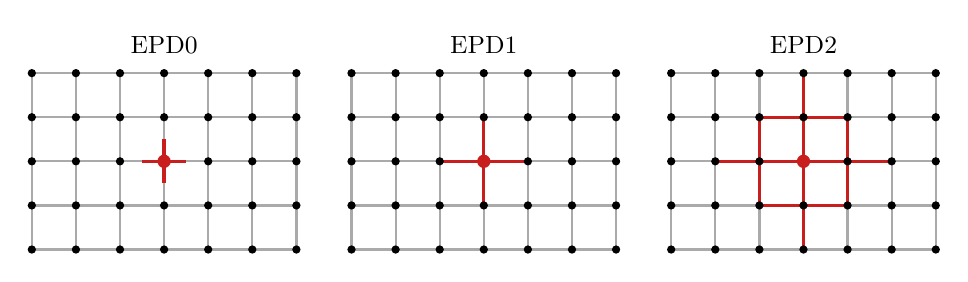
\begin{tikzpicture}
\draw[highc,thick] (0.000,0.000) -- (0.000,0.280);
\draw[highc,thick] (0.000,0.560) -- (0.000,0.280);
\draw[highc,thick] (0.000,0.000) -- (0.280,0.000);
\draw[highc,thick] (0.560,0.000) -- (0.280,0.000);
\draw[highc,thick] (0.000,0.560) -- (0.000,0.840);
\draw[highc,thick] (0.000,1.120) -- (0.000,0.840);
\draw[highc,thick] (0.000,0.560) -- (0.280,0.560);
\draw[highc,thick] (0.560,0.560) -- (0.280,0.560);
\draw[highc,thick] (0.000,1.120) -- (0.000,1.400);
\draw[highc,thick] (0.000,1.680) -- (0.000,1.400);
\draw[highc,thick] (0.000,1.120) -- (0.280,1.120);
\draw[highc,thick] (0.560,1.120) -- (0.280,1.120);
\draw[highc,thick] (0.000,1.680) -- (0.000,1.960);
\draw[highc,thick] (0.000,2.240) -- (0.000,1.960);
\draw[highc,thick] (0.000,1.680) -- (0.280,1.680);
\draw[highc,thick] (0.560,1.680) -- (0.280,1.680);
\draw[highc,thick] (0.000,2.240) -- (0.280,2.240);
\draw[highc,thick] (0.560,2.240) -- (0.280,2.240);
\draw[highc,thick] (0.560,0.000) -- (0.560,0.280);
\draw[highc,thick] (0.560,0.560) -- (0.560,0.280);
\draw[highc,thick] (0.560,0.000) -- (0.840,0.000);
\draw[highc,thick] (1.120,0.000) -- (0.840,0.000);
\draw[highc,thick] (0.560,0.560) -- (0.560,0.840);
\draw[highc,thick] (0.560,1.120) -- (0.560,0.840);
\draw[highc,thick] (0.560,0.560) -- (0.840,0.560);
\draw[highc,thick] (1.120,0.560) -- (0.840,0.560);
\draw[highc,thick] (0.560,1.120) -- (0.560,1.400);
\draw[highc,thick] (0.560,1.680) -- (0.560,1.400);
\draw[highc,thick] (0.560,1.120) -- (0.840,1.120);
\draw[highc,thick] (1.120,1.120) -- (0.840,1.120);
\draw[highc,thick] (0.560,1.680) -- (0.560,1.960);
\draw[highc,thick] (0.560,2.240) -- (0.560,1.960);
\draw[highc,thick] (0.560,1.680) -- (0.840,1.680);
\draw[highc,thick] (1.120,1.680) -- (0.840,1.680);
\draw[highc,thick] (0.560,2.240) -- (0.840,2.240);
\draw[highc,thick] (1.120,2.240) -- (0.840,2.240);
\draw[highc,thick] (1.120,0.000) -- (1.120,0.280);
\draw[highc,thick] (1.120,0.560) -- (1.120,0.280);
\draw[highc,thick] (1.120,0.000) -- (1.400,0.000);
\draw[highc,thick] (1.680,0.000) -- (1.400,0.000);
\draw[highc,thick] (1.120,0.560) -- (1.120,0.840);
\draw[highc,thick] (1.120,1.120) -- (1.120,0.840);
\draw[highc,thick] (1.120,0.560) -- (1.400,0.560);
\draw[highc,thick] (1.680,0.560) -- (1.400,0.560);
\draw[highc,thick] (1.120,1.120) -- (1.120,1.400);
\draw[highc,thick] (1.120,1.680) -- (1.120,1.400);
\draw[highc,thick] (1.120,1.120) -- (1.400,1.120);
\draw[lowc,very thick] (1.680,1.120) -- (1.400,1.120);
\draw[highc,thick] (1.120,1.680) -- (1.120,1.960);
\draw[highc,thick] (1.120,2.240) -- (1.120,1.960);
\draw[highc,thick] (1.120,1.680) -- (1.400,1.680);
\draw[highc,thick] (1.680,1.680) -- (1.400,1.680);
\draw[highc,thick] (1.120,2.240) -- (1.400,2.240);
\draw[highc,thick] (1.680,2.240) -- (1.400,2.240);
\draw[highc,thick] (1.680,0.000) -- (1.680,0.280);
\draw[highc,thick] (1.680,0.560) -- (1.680,0.280);
\draw[highc,thick] (1.680,0.000) -- (1.960,0.000);
\draw[highc,thick] (2.240,0.000) -- (1.960,0.000);
\draw[highc,thick] (1.680,0.560) -- (1.680,0.840);
\draw[lowc,very thick] (1.680,1.120) -- (1.680,0.840);
\draw[highc,thick] (1.680,0.560) -- (1.960,0.560);
\draw[highc,thick] (2.240,0.560) -- (1.960,0.560);
\draw[lowc,very thick] (1.680,1.120) -- (1.680,1.400);
\draw[highc,thick] (1.680,1.680) -- (1.680,1.400);
\draw[lowc,very thick] (1.680,1.120) -- (1.960,1.120);
\draw[highc,thick] (2.240,1.120) -- (1.960,1.120);
\draw[highc,thick] (1.680,1.680) -- (1.680,1.960);
\draw[highc,thick] (1.680,2.240) -- (1.680,1.960);
\draw[highc,thick] (1.680,1.680) -- (1.960,1.680);
\draw[highc,thick] (2.240,1.680) -- (1.960,1.680);
\draw[highc,thick] (1.680,2.240) -- (1.960,2.240);
\draw[highc,thick] (2.240,2.240) -- (1.960,2.240);
\draw[highc,thick] (2.240,0.000) -- (2.240,0.280);
\draw[highc,thick] (2.240,0.560) -- (2.240,0.280);
\draw[highc,thick] (2.240,0.000) -- (2.520,0.000);
\draw[highc,thick] (2.800,0.000) -- (2.520,0.000);
\draw[highc,thick] (2.240,0.560) -- (2.240,0.840);
\draw[highc,thick] (2.240,1.120) -- (2.240,0.840);
\draw[highc,thick] (2.240,0.560) -- (2.520,0.560);
\draw[highc,thick] (2.800,0.560) -- (2.520,0.560);
\draw[highc,thick] (2.240,1.120) -- (2.240,1.400);
\draw[highc,thick] (2.240,1.680) -- (2.240,1.400);
\draw[highc,thick] (2.240,1.120) -- (2.520,1.120);
\draw[highc,thick] (2.800,1.120) -- (2.520,1.120);
\draw[highc,thick] (2.240,1.680) -- (2.240,1.960);
\draw[highc,thick] (2.240,2.240) -- (2.240,1.960);
\draw[highc,thick] (2.240,1.680) -- (2.520,1.680);
\draw[highc,thick] (2.800,1.680) -- (2.520,1.680);
\draw[highc,thick] (2.240,2.240) -- (2.520,2.240);
\draw[highc,thick] (2.800,2.240) -- (2.520,2.240);
\draw[highc,thick] (2.800,0.000) -- (2.800,0.280);
\draw[highc,thick] (2.800,0.560) -- (2.800,0.280);
\draw[highc,thick] (2.800,0.000) -- (3.080,0.000);
\draw[highc,thick] (3.360,0.000) -- (3.080,0.000);
\draw[highc,thick] (2.800,0.560) -- (2.800,0.840);
\draw[highc,thick] (2.800,1.120) -- (2.800,0.840);
\draw[highc,thick] (2.800,0.560) -- (3.080,0.560);
\draw[highc,thick] (3.360,0.560) -- (3.080,0.560);
\draw[highc,thick] (2.800,1.120) -- (2.800,1.400);
\draw[highc,thick] (2.800,1.680) -- (2.800,1.400);
\draw[highc,thick] (2.800,1.120) -- (3.080,1.120);
\draw[highc,thick] (3.360,1.120) -- (3.080,1.120);
\draw[highc,thick] (2.800,1.680) -- (2.800,1.960);
\draw[highc,thick] (2.800,2.240) -- (2.800,1.960);
\draw[highc,thick] (2.800,1.680) -- (3.080,1.680);
\draw[highc,thick] (3.360,1.680) -- (3.080,1.680);
\draw[highc,thick] (2.800,2.240) -- (3.080,2.240);
\draw[highc,thick] (3.360,2.240) -- (3.080,2.240);
\draw[highc,thick] (3.360,0.000) -- (3.360,0.280);
\draw[highc,thick] (3.360,0.560) -- (3.360,0.280);
\draw[highc,thick] (3.360,0.560) -- (3.360,0.840);
\draw[highc,thick] (3.360,1.120) -- (3.360,0.840);
\draw[highc,thick] (3.360,1.120) -- (3.360,1.400);
\draw[highc,thick] (3.360,1.680) -- (3.360,1.400);
\draw[highc,thick] (3.360,1.680) -- (3.360,1.960);
\draw[highc,thick] (3.360,2.240) -- (3.360,1.960);
\fill[black] (0.000,0.000) circle (1.5pt);
\fill[black] (0.000,0.560) circle (1.5pt);
\fill[black] (0.000,1.120) circle (1.5pt);
\fill[black] (0.000,1.680) circle (1.5pt);
\fill[black] (0.000,2.240) circle (1.5pt);
\fill[black] (0.560,0.000) circle (1.5pt);
\fill[black] (0.560,0.560) circle (1.5pt);
\fill[black] (0.560,1.120) circle (1.5pt);
\fill[black] (0.560,1.680) circle (1.5pt);
\fill[black] (0.560,2.240) circle (1.5pt);
\fill[black] (1.120,0.000) circle (1.5pt);
\fill[black] (1.120,0.560) circle (1.5pt);
\fill[black] (1.120,1.120) circle (1.5pt);
\fill[black] (1.120,1.680) circle (1.5pt);
\fill[black] (1.120,2.240) circle (1.5pt);
\fill[black] (1.680,0.000) circle (1.5pt);
\fill[black] (1.680,0.560) circle (1.5pt);
\fill[lowc] (1.680,1.120) circle (2.4pt);
\fill[black] (1.680,1.680) circle (1.5pt);
\fill[black] (1.680,2.240) circle (1.5pt);
\fill[black] (2.240,0.000) circle (1.5pt);
\fill[black] (2.240,0.560) circle (1.5pt);
\fill[black] (2.240,1.120) circle (1.5pt);
\fill[black] (2.240,1.680) circle (1.5pt);
\fill[black] (2.240,2.240) circle (1.5pt);
\fill[black] (2.800,0.000) circle (1.5pt);
\fill[black] (2.800,0.560) circle (1.5pt);
\fill[black] (2.800,1.120) circle (1.5pt);
\fill[black] (2.800,1.680) circle (1.5pt);
\fill[black] (2.800,2.240) circle (1.5pt);
\fill[black] (3.360,0.000) circle (1.5pt);
\fill[black] (3.360,0.560) circle (1.5pt);
\fill[black] (3.360,1.120) circle (1.5pt);
\fill[black] (3.360,1.680) circle (1.5pt);
\fill[black] (3.360,2.240) circle (1.5pt);
\node[anchor=south] at (1.680,2.360) {\small EPD0};
\draw[highc,thick] (4.060,0.000) -- (4.060,0.280);
\draw[highc,thick] (4.060,0.560) -- (4.060,0.280);
\draw[highc,thick] (4.060,0.000) -- (4.340,0.000);
\draw[highc,thick] (4.620,0.000) -- (4.340,0.000);
\draw[highc,thick] (4.060,0.560) -- (4.060,0.840);
\draw[highc,thick] (4.060,1.120) -- (4.060,0.840);
\draw[highc,thick] (4.060,0.560) -- (4.340,0.560);
\draw[highc,thick] (4.620,0.560) -- (4.340,0.560);
\draw[highc,thick] (4.060,1.120) -- (4.060,1.400);
\draw[highc,thick] (4.060,1.680) -- (4.060,1.400);
\draw[highc,thick] (4.060,1.120) -- (4.340,1.120);
\draw[highc,thick] (4.620,1.120) -- (4.340,1.120);
\draw[highc,thick] (4.060,1.680) -- (4.060,1.960);
\draw[highc,thick] (4.060,2.240) -- (4.060,1.960);
\draw[highc,thick] (4.060,1.680) -- (4.340,1.680);
\draw[highc,thick] (4.620,1.680) -- (4.340,1.680);
\draw[highc,thick] (4.060,2.240) -- (4.340,2.240);
\draw[highc,thick] (4.620,2.240) -- (4.340,2.240);
\draw[highc,thick] (4.620,0.000) -- (4.620,0.280);
\draw[highc,thick] (4.620,0.560) -- (4.620,0.280);
\draw[highc,thick] (4.620,0.000) -- (4.900,0.000);
\draw[highc,thick] (5.180,0.000) -- (4.900,0.000);
\draw[highc,thick] (4.620,0.560) -- (4.620,0.840);
\draw[highc,thick] (4.620,1.120) -- (4.620,0.840);
\draw[highc,thick] (4.620,0.560) -- (4.900,0.560);
\draw[highc,thick] (5.180,0.560) -- (4.900,0.560);
\draw[highc,thick] (4.620,1.120) -- (4.620,1.400);
\draw[highc,thick] (4.620,1.680) -- (4.620,1.400);
\draw[highc,thick] (4.620,1.120) -- (4.900,1.120);
\draw[highc,thick] (5.180,1.120) -- (4.900,1.120);
\draw[highc,thick] (4.620,1.680) -- (4.620,1.960);
\draw[highc,thick] (4.620,2.240) -- (4.620,1.960);
\draw[highc,thick] (4.620,1.680) -- (4.900,1.680);
\draw[highc,thick] (5.180,1.680) -- (4.900,1.680);
\draw[highc,thick] (4.620,2.240) -- (4.900,2.240);
\draw[highc,thick] (5.180,2.240) -- (4.900,2.240);
\draw[highc,thick] (5.180,0.000) -- (5.180,0.280);
\draw[highc,thick] (5.180,0.560) -- (5.180,0.280);
\draw[highc,thick] (5.180,0.000) -- (5.460,0.000);
\draw[highc,thick] (5.740,0.000) -- (5.460,0.000);
\draw[highc,thick] (5.180,0.560) -- (5.180,0.840);
\draw[highc,thick] (5.180,1.120) -- (5.180,0.840);
\draw[highc,thick] (5.180,0.560) -- (5.460,0.560);
\draw[highc,thick] (5.740,0.560) -- (5.460,0.560);
\draw[highc,thick] (5.180,1.120) -- (5.180,1.400);
\draw[highc,thick] (5.180,1.680) -- (5.180,1.400);
\draw[lowc,very thick] (5.180,1.120) -- (5.460,1.120);
\draw[lowc,very thick] (5.740,1.120) -- (5.460,1.120);
\draw[highc,thick] (5.180,1.680) -- (5.180,1.960);
\draw[highc,thick] (5.180,2.240) -- (5.180,1.960);
\draw[highc,thick] (5.180,1.680) -- (5.460,1.680);
\draw[highc,thick] (5.740,1.680) -- (5.460,1.680);
\draw[highc,thick] (5.180,2.240) -- (5.460,2.240);
\draw[highc,thick] (5.740,2.240) -- (5.460,2.240);
\draw[highc,thick] (5.740,0.000) -- (5.740,0.280);
\draw[highc,thick] (5.740,0.560) -- (5.740,0.280);
\draw[highc,thick] (5.740,0.000) -- (6.020,0.000);
\draw[highc,thick] (6.300,0.000) -- (6.020,0.000);
\draw[lowc,very thick] (5.740,0.560) -- (5.740,0.840);
\draw[lowc,very thick] (5.740,1.120) -- (5.740,0.840);
\draw[highc,thick] (5.740,0.560) -- (6.020,0.560);
\draw[highc,thick] (6.300,0.560) -- (6.020,0.560);
\draw[lowc,very thick] (5.740,1.120) -- (5.740,1.400);
\draw[lowc,very thick] (5.740,1.680) -- (5.740,1.400);
\draw[lowc,very thick] (5.740,1.120) -- (6.020,1.120);
\draw[lowc,very thick] (6.300,1.120) -- (6.020,1.120);
\draw[highc,thick] (5.740,1.680) -- (5.740,1.960);
\draw[highc,thick] (5.740,2.240) -- (5.740,1.960);
\draw[highc,thick] (5.740,1.680) -- (6.020,1.680);
\draw[highc,thick] (6.300,1.680) -- (6.020,1.680);
\draw[highc,thick] (5.740,2.240) -- (6.020,2.240);
\draw[highc,thick] (6.300,2.240) -- (6.020,2.240);
\draw[highc,thick] (6.300,0.000) -- (6.300,0.280);
\draw[highc,thick] (6.300,0.560) -- (6.300,0.280);
\draw[highc,thick] (6.300,0.000) -- (6.580,0.000);
\draw[highc,thick] (6.860,0.000) -- (6.580,0.000);
\draw[highc,thick] (6.300,0.560) -- (6.300,0.840);
\draw[highc,thick] (6.300,1.120) -- (6.300,0.840);
\draw[highc,thick] (6.300,0.560) -- (6.580,0.560);
\draw[highc,thick] (6.860,0.560) -- (6.580,0.560);
\draw[highc,thick] (6.300,1.120) -- (6.300,1.400);
\draw[highc,thick] (6.300,1.680) -- (6.300,1.400);
\draw[highc,thick] (6.300,1.120) -- (6.580,1.120);
\draw[highc,thick] (6.860,1.120) -- (6.580,1.120);
\draw[highc,thick] (6.300,1.680) -- (6.300,1.960);
\draw[highc,thick] (6.300,2.240) -- (6.300,1.960);
\draw[highc,thick] (6.300,1.680) -- (6.580,1.680);
\draw[highc,thick] (6.860,1.680) -- (6.580,1.680);
\draw[highc,thick] (6.300,2.240) -- (6.580,2.240);
\draw[highc,thick] (6.860,2.240) -- (6.580,2.240);
\draw[highc,thick] (6.860,0.000) -- (6.860,0.280);
\draw[highc,thick] (6.860,0.560) -- (6.860,0.280);
\draw[highc,thick] (6.860,0.000) -- (7.140,0.000);
\draw[highc,thick] (7.420,0.000) -- (7.140,0.000);
\draw[highc,thick] (6.860,0.560) -- (6.860,0.840);
\draw[highc,thick] (6.860,1.120) -- (6.860,0.840);
\draw[highc,thick] (6.860,0.560) -- (7.140,0.560);
\draw[highc,thick] (7.420,0.560) -- (7.140,0.560);
\draw[highc,thick] (6.860,1.120) -- (6.860,1.400);
\draw[highc,thick] (6.860,1.680) -- (6.860,1.400);
\draw[highc,thick] (6.860,1.120) -- (7.140,1.120);
\draw[highc,thick] (7.420,1.120) -- (7.140,1.120);
\draw[highc,thick] (6.860,1.680) -- (6.860,1.960);
\draw[highc,thick] (6.860,2.240) -- (6.860,1.960);
\draw[highc,thick] (6.860,1.680) -- (7.140,1.680);
\draw[highc,thick] (7.420,1.680) -- (7.140,1.680);
\draw[highc,thick] (6.860,2.240) -- (7.140,2.240);
\draw[highc,thick] (7.420,2.240) -- (7.140,2.240);
\draw[highc,thick] (7.420,0.000) -- (7.420,0.280);
\draw[highc,thick] (7.420,0.560) -- (7.420,0.280);
\draw[highc,thick] (7.420,0.560) -- (7.420,0.840);
\draw[highc,thick] (7.420,1.120) -- (7.420,0.840);
\draw[highc,thick] (7.420,1.120) -- (7.420,1.400);
\draw[highc,thick] (7.420,1.680) -- (7.420,1.400);
\draw[highc,thick] (7.420,1.680) -- (7.420,1.960);
\draw[highc,thick] (7.420,2.240) -- (7.420,1.960);
\fill[black] (4.060,0.000) circle (1.5pt);
\fill[black] (4.060,0.560) circle (1.5pt);
\fill[black] (4.060,1.120) circle (1.5pt);
\fill[black] (4.060,1.680) circle (1.5pt);
\fill[black] (4.060,2.240) circle (1.5pt);
\fill[black] (4.620,0.000) circle (1.5pt);
\fill[black] (4.620,0.560) circle (1.5pt);
\fill[black] (4.620,1.120) circle (1.5pt);
\fill[black] (4.620,1.680) circle (1.5pt);
\fill[black] (4.620,2.240) circle (1.5pt);
\fill[black] (5.180,0.000) circle (1.5pt);
\fill[black] (5.180,0.560) circle (1.5pt);
\fill[black] (5.180,1.120) circle (1.5pt);
\fill[black] (5.180,1.680) circle (1.5pt);
\fill[black] (5.180,2.240) circle (1.5pt);
\fill[black] (5.740,0.000) circle (1.5pt);
\fill[black] (5.740,0.560) circle (1.5pt);
\fill[lowc] (5.740,1.120) circle (2.4pt);
\fill[black] (5.740,1.680) circle (1.5pt);
\fill[black] (5.740,2.240) circle (1.5pt);
\fill[black] (6.300,0.000) circle (1.5pt);
\fill[black] (6.300,0.560) circle (1.5pt);
\fill[black] (6.300,1.120) circle (1.5pt);
\fill[black] (6.300,1.680) circle (1.5pt);
\fill[black] (6.300,2.240) circle (1.5pt);
\fill[black] (6.860,0.000) circle (1.5pt);
\fill[black] (6.860,0.560) circle (1.5pt);
\fill[black] (6.860,1.120) circle (1.5pt);
\fill[black] (6.860,1.680) circle (1.5pt);
\fill[black] (6.860,2.240) circle (1.5pt);
\fill[black] (7.420,0.000) circle (1.5pt);
\fill[black] (7.420,0.560) circle (1.5pt);
\fill[black] (7.420,1.120) circle (1.5pt);
\fill[black] (7.420,1.680) circle (1.5pt);
\fill[black] (7.420,2.240) circle (1.5pt);
\node[anchor=south] at (5.740,2.360) {\small EPD1};
\draw[highc,thick] (8.120,0.000) -- (8.120,0.280);
\draw[highc,thick] (8.120,0.560) -- (8.120,0.280);
\draw[highc,thick] (8.120,0.000) -- (8.400,0.000);
\draw[highc,thick] (8.680,0.000) -- (8.400,0.000);
\draw[highc,thick] (8.120,0.560) -- (8.120,0.840);
\draw[highc,thick] (8.120,1.120) -- (8.120,0.840);
\draw[highc,thick] (8.120,0.560) -- (8.400,0.560);
\draw[highc,thick] (8.680,0.560) -- (8.400,0.560);
\draw[highc,thick] (8.120,1.120) -- (8.120,1.400);
\draw[highc,thick] (8.120,1.680) -- (8.120,1.400);
\draw[highc,thick] (8.120,1.120) -- (8.400,1.120);
\draw[highc,thick] (8.680,1.120) -- (8.400,1.120);
\draw[highc,thick] (8.120,1.680) -- (8.120,1.960);
\draw[highc,thick] (8.120,2.240) -- (8.120,1.960);
\draw[highc,thick] (8.120,1.680) -- (8.400,1.680);
\draw[highc,thick] (8.680,1.680) -- (8.400,1.680);
\draw[highc,thick] (8.120,2.240) -- (8.400,2.240);
\draw[highc,thick] (8.680,2.240) -- (8.400,2.240);
\draw[highc,thick] (8.680,0.000) -- (8.680,0.280);
\draw[highc,thick] (8.680,0.560) -- (8.680,0.280);
\draw[highc,thick] (8.680,0.000) -- (8.960,0.000);
\draw[highc,thick] (9.240,0.000) -- (8.960,0.000);
\draw[highc,thick] (8.680,0.560) -- (8.680,0.840);
\draw[highc,thick] (8.680,1.120) -- (8.680,0.840);
\draw[highc,thick] (8.680,0.560) -- (8.960,0.560);
\draw[highc,thick] (9.240,0.560) -- (8.960,0.560);
\draw[highc,thick] (8.680,1.120) -- (8.680,1.400);
\draw[highc,thick] (8.680,1.680) -- (8.680,1.400);
\draw[lowc,very thick] (8.680,1.120) -- (8.960,1.120);
\draw[lowc,very thick] (9.240,1.120) -- (8.960,1.120);
\draw[highc,thick] (8.680,1.680) -- (8.680,1.960);
\draw[highc,thick] (8.680,2.240) -- (8.680,1.960);
\draw[highc,thick] (8.680,1.680) -- (8.960,1.680);
\draw[highc,thick] (9.240,1.680) -- (8.960,1.680);
\draw[highc,thick] (8.680,2.240) -- (8.960,2.240);
\draw[highc,thick] (9.240,2.240) -- (8.960,2.240);
\draw[highc,thick] (9.240,0.000) -- (9.240,0.280);
\draw[highc,thick] (9.240,0.560) -- (9.240,0.280);
\draw[highc,thick] (9.240,0.000) -- (9.520,0.000);
\draw[highc,thick] (9.800,0.000) -- (9.520,0.000);
\draw[lowc,very thick] (9.240,0.560) -- (9.240,0.840);
\draw[lowc,very thick] (9.240,1.120) -- (9.240,0.840);
\draw[lowc,very thick] (9.240,0.560) -- (9.520,0.560);
\draw[lowc,very thick] (9.800,0.560) -- (9.520,0.560);
\draw[lowc,very thick] (9.240,1.120) -- (9.240,1.400);
\draw[lowc,very thick] (9.240,1.680) -- (9.240,1.400);
\draw[lowc,very thick] (9.240,1.120) -- (9.520,1.120);
\draw[lowc,very thick] (9.800,1.120) -- (9.520,1.120);
\draw[highc,thick] (9.240,1.680) -- (9.240,1.960);
\draw[highc,thick] (9.240,2.240) -- (9.240,1.960);
\draw[lowc,very thick] (9.240,1.680) -- (9.520,1.680);
\draw[lowc,very thick] (9.800,1.680) -- (9.520,1.680);
\draw[highc,thick] (9.240,2.240) -- (9.520,2.240);
\draw[highc,thick] (9.800,2.240) -- (9.520,2.240);
\draw[lowc,very thick] (9.800,0.000) -- (9.800,0.280);
\draw[lowc,very thick] (9.800,0.560) -- (9.800,0.280);
\draw[highc,thick] (9.800,0.000) -- (10.080,0.000);
\draw[highc,thick] (10.360,0.000) -- (10.080,0.000);
\draw[lowc,very thick] (9.800,0.560) -- (9.800,0.840);
\draw[lowc,very thick] (9.800,1.120) -- (9.800,0.840);
\draw[lowc,very thick] (9.800,0.560) -- (10.080,0.560);
\draw[lowc,very thick] (10.360,0.560) -- (10.080,0.560);
\draw[lowc,very thick] (9.800,1.120) -- (9.800,1.400);
\draw[lowc,very thick] (9.800,1.680) -- (9.800,1.400);
\draw[lowc,very thick] (9.800,1.120) -- (10.080,1.120);
\draw[lowc,very thick] (10.360,1.120) -- (10.080,1.120);
\draw[lowc,very thick] (9.800,1.680) -- (9.800,1.960);
\draw[lowc,very thick] (9.800,2.240) -- (9.800,1.960);
\draw[lowc,very thick] (9.800,1.680) -- (10.080,1.680);
\draw[lowc,very thick] (10.360,1.680) -- (10.080,1.680);
\draw[highc,thick] (9.800,2.240) -- (10.080,2.240);
\draw[highc,thick] (10.360,2.240) -- (10.080,2.240);
\draw[highc,thick] (10.360,0.000) -- (10.360,0.280);
\draw[highc,thick] (10.360,0.560) -- (10.360,0.280);
\draw[highc,thick] (10.360,0.000) -- (10.640,0.000);
\draw[highc,thick] (10.920,0.000) -- (10.640,0.000);
\draw[lowc,very thick] (10.360,0.560) -- (10.360,0.840);
\draw[lowc,very thick] (10.360,1.120) -- (10.360,0.840);
\draw[highc,thick] (10.360,0.560) -- (10.640,0.560);
\draw[highc,thick] (10.920,0.560) -- (10.640,0.560);
\draw[lowc,very thick] (10.360,1.120) -- (10.360,1.400);
\draw[lowc,very thick] (10.360,1.680) -- (10.360,1.400);
\draw[lowc,very thick] (10.360,1.120) -- (10.640,1.120);
\draw[lowc,very thick] (10.920,1.120) -- (10.640,1.120);
\draw[highc,thick] (10.360,1.680) -- (10.360,1.960);
\draw[highc,thick] (10.360,2.240) -- (10.360,1.960);
\draw[highc,thick] (10.360,1.680) -- (10.640,1.680);
\draw[highc,thick] (10.920,1.680) -- (10.640,1.680);
\draw[highc,thick] (10.360,2.240) -- (10.640,2.240);
\draw[highc,thick] (10.920,2.240) -- (10.640,2.240);
\draw[highc,thick] (10.920,0.000) -- (10.920,0.280);
\draw[highc,thick] (10.920,0.560) -- (10.920,0.280);
\draw[highc,thick] (10.920,0.000) -- (11.200,0.000);
\draw[highc,thick] (11.480,0.000) -- (11.200,0.000);
\draw[highc,thick] (10.920,0.560) -- (10.920,0.840);
\draw[highc,thick] (10.920,1.120) -- (10.920,0.840);
\draw[highc,thick] (10.920,0.560) -- (11.200,0.560);
\draw[highc,thick] (11.480,0.560) -- (11.200,0.560);
\draw[highc,thick] (10.920,1.120) -- (10.920,1.400);
\draw[highc,thick] (10.920,1.680) -- (10.920,1.400);
\draw[highc,thick] (10.920,1.120) -- (11.200,1.120);
\draw[highc,thick] (11.480,1.120) -- (11.200,1.120);
\draw[highc,thick] (10.920,1.680) -- (10.920,1.960);
\draw[highc,thick] (10.920,2.240) -- (10.920,1.960);
\draw[highc,thick] (10.920,1.680) -- (11.200,1.680);
\draw[highc,thick] (11.480,1.680) -- (11.200,1.680);
\draw[highc,thick] (10.920,2.240) -- (11.200,2.240);
\draw[highc,thick] (11.480,2.240) -- (11.200,2.240);
\draw[highc,thick] (11.480,0.000) -- (11.480,0.280);
\draw[highc,thick] (11.480,0.560) -- (11.480,0.280);
\draw[highc,thick] (11.480,0.560) -- (11.480,0.840);
\draw[highc,thick] (11.480,1.120) -- (11.480,0.840);
\draw[highc,thick] (11.480,1.120) -- (11.480,1.400);
\draw[highc,thick] (11.480,1.680) -- (11.480,1.400);
\draw[highc,thick] (11.480,1.680) -- (11.480,1.960);
\draw[highc,thick] (11.480,2.240) -- (11.480,1.960);
\fill[black] (8.120,0.000) circle (1.5pt);
\fill[black] (8.120,0.560) circle (1.5pt);
\fill[black] (8.120,1.120) circle (1.5pt);
\fill[black] (8.120,1.680) circle (1.5pt);
\fill[black] (8.120,2.240) circle (1.5pt);
\fill[black] (8.680,0.000) circle (1.5pt);
\fill[black] (8.680,0.560) circle (1.5pt);
\fill[black] (8.680,1.120) circle (1.5pt);
\fill[black] (8.680,1.680) circle (1.5pt);
\fill[black] (8.680,2.240) circle (1.5pt);
\fill[black] (9.240,0.000) circle (1.5pt);
\fill[black] (9.240,0.560) circle (1.5pt);
\fill[black] (9.240,1.120) circle (1.5pt);
\fill[black] (9.240,1.680) circle (1.5pt);
\fill[black] (9.240,2.240) circle (1.5pt);
\fill[black] (9.800,0.000) circle (1.5pt);
\fill[black] (9.800,0.560) circle (1.5pt);
\fill[lowc] (9.800,1.120) circle (2.4pt);
\fill[black] (9.800,1.680) circle (1.5pt);
\fill[black] (9.800,2.240) circle (1.5pt);
\fill[black] (10.360,0.000) circle (1.5pt);
\fill[black] (10.360,0.560) circle (1.5pt);
\fill[black] (10.360,1.120) circle (1.5pt);
\fill[black] (10.360,1.680) circle (1.5pt);
\fill[black] (10.360,2.240) circle (1.5pt);
\fill[black] (10.920,0.000) circle (1.5pt);
\fill[black] (10.920,0.560) circle (1.5pt);
\fill[black] (10.920,1.120) circle (1.5pt);
\fill[black] (10.920,1.680) circle (1.5pt);
\fill[black] (10.920,2.240) circle (1.5pt);
\fill[black] (11.480,0.000) circle (1.5pt);
\fill[black] (11.480,0.560) circle (1.5pt);
\fill[black] (11.480,1.120) circle (1.5pt);
\fill[black] (11.480,1.680) circle (1.5pt);
\fill[black] (11.480,2.240) circle (1.5pt);
\node[anchor=south] at (9.800,2.360) {\small EPD2};
\end{tikzpicture}

\caption{Interface orders for one particle (filled red) lowered to order one in a high-order region, on a lattice patch with nearest-neighbour edges standing in for the neighbour graph. The half of an edge next to a particle shows the order with which this particle's reconstruction enters the interface: red for order one, grey for the full order.}\label{fig:epd}
\end{figure}

\begin{proposition}[Fallback property]\label{prop:fallback}
Let $i\in I$ have order $k_i=1$. Under EPD1 and EPD2, $\Lop_i$ coincides with a first-order operator, i.e.\ \eqref{eq:scheme} with piecewise constant interface states on all edges of $i$: with the derivative weights of degree $q_i$ (\cref{rem:safeguards}), i.e.\ degree one in the coupled mode and $\qdiv(k_{\mathrm{div}})$ in the frozen mode unless a safeguard lowers it. If $K=1$, this holds under every rule. Under EPD0 with $K\ge2$ it does not hold in general.
\end{proposition}

\begin{proof}
Under EPD1, $\ord ij=\ord ji=\min\{1,k_j\}=1$ for all $j\in\nb(i)$; under EPD2 the minimum runs over a set that contains $i$. For $K=1$ all orders are one. In all cases \eqref{eq:states} gives piecewise constant states, and the coupled mode gives $q_i=\qdiv(1)=1$, the frozen mode $q_i=\qdiv(k_{\mathrm{div}})$. Under EPD0, $\ord ji=k_j$ may exceed one, so that $U_{ji}\ne U_j$.
\end{proof}

The failure of EPD0 is consistent with FV MOOD \cite{Clain2011}, where the polynomial degree used at a face is the minimum of the degrees of the two adjacent cells, so that a cell decremented to the lowest degree is advanced by the first-order scheme (called the parachute scheme in later MOOD papers); EPD1 is this rule on the edges of the neighbour graph.

Combining \cref{prop:fallback} with \cref{cor:aligned} gives the local statement that the time integration needs.

\begin{proposition}[Local admissibility at order one]\label{prop:local}
Let $\Ad$ and the fluxes satisfy the hypotheses of \cref{prop:positivity}. Let $i\in I$ have order $k_i=1$, under EPD1 or EPD2, or under any rule if $K=1$. Use the aligned Rusanov flux, in either divergence mode, with signs taken from the weights in use (\cref{rem:signs}), and let the derivative fit of $i$ be unregularized on a $\Pi_{q_i}$-unisolvent neighbourhood. Let $Y\in\Ad$ at all $l\in\cnb(i)$, ghost neighbours included, and let $\tau>0$ satisfy \eqref{eq:cflpos} with $s_{ij,d}=\max\{\lambda_d(Y_i),\lambda_d(Y_j)\}$, where $s_{ij,d}>0$ wherever $c^{(d)}_{ij}\ne0$ (automatic for the Euler equations). Then $Y_i+\tau\,\Lop_i(Y)\in\Ad$.
\end{proposition}

\begin{proof}
By \cref{prop:fallback}, $\Lop_i$ is the first-order operator with the weights of degree $q_i$. Since $k_i=1$, either $k_i<K$ or $K=1$, so all edges of $i$ are aligned and \cref{cor:aligned} gives (a) and (b) of \cref{prop:positivity}, which yields the claim.
\end{proof}

% ===========================================================================
\section{Time integration and stage-wise MOOD}\label{sec:time}
% ===========================================================================

\subsection{Explicit Runge--Kutta methods and their canonical Shu--Osher form}

The semi-discrete system \eqref{eq:scheme} is integrated with an explicit $s$-stage Runge--Kutta method in Butcher form,
\begin{equation}\label{eq:rk}
Y_k = U^n+\Delta t\sum_{l<k}a_{kl}\,K_l,\quad K_l=\Lop(Y_l),\quad k=1,\dots,s,\qquad Y_{s+1}:=U^{n+1}=U^n+\Delta t\sum_{l=1}^sb_l\,K_l,
\end{equation}
where the boundary operator sets the ghost states of every stage $Y_k$ and of $U^{n+1}$ from their interior states. Let $\hat A\in\R^{(s+1)\times(s+1)}$ be the strictly lower triangular matrix with the rows $(a_{k1},\dots,a_{k,k-1},0,\dots,0)$, $k\le s$, and the last row $(b_1,\dots,b_s,0)$. Following \cite{Ketcheson2008,GottliebKetchesonShu2011}, for $r>0$ let
\begin{equation}\label{eq:canonical}
\alpha^{(r)}=r\hat A\,(\mathrm{Id}+r\hat A)^{-1},\qquad v^{(r)}=(\mathrm{Id}-\alpha^{(r)})\,e,\qquad e=(1,\dots,1)^{\mathsf T}.
\end{equation}

\begin{lemma}[Canonical Shu--Osher form]\label{lem:canonical}
For every $r>0$, $\alpha^{(r)}$ is strictly lower triangular, $v^{(r)}_k+\sum_j\alpha^{(r)}_{kj}=1$ for all $k$, and the interior states of \eqref{eq:rk} satisfy
\begin{equation}\label{eq:shuosher}
Y_k=v^{(r)}_k\,U^n+\sum_{j<k}\alpha^{(r)}_{kj}\,W_j,\qquad W_j:=Y_j+\frac{\Delta t}{r}\,\Lop(Y_j),\qquad k=1,\dots,s+1 .
\end{equation}
\end{lemma}

\begin{proof}
Stack the interior stage values as $\mathbf Y=(Y_1,\dots,Y_{s+1})$ and set $\Lop(\mathbf Y)=(\Lop(Y_1),\dots,\Lop(Y_{s+1}))$; the last entry is multiplied by the zero last column of $\hat A$. Then \eqref{eq:rk} reads $\mathbf Y=e\,U^n+\Delta t\,\hat A\,\Lop(\mathbf Y)$, hence $(\mathrm{Id}+r\hat A)\mathbf Y=e\,U^n+r\hat A\big(\mathbf Y+\tfrac{\Delta t}{r}\Lop(\mathbf Y)\big)$. The matrix $\mathrm{Id}+r\hat A$ is unit lower triangular and invertible, and $(\mathrm{Id}+r\hat A)^{-1}=\mathrm{Id}-r\hat A(\mathrm{Id}+r\hat A)^{-1}=\mathrm{Id}-\alpha^{(r)}$. Multiplying by it gives \eqref{eq:shuosher}, with $v^{(r)}=(\mathrm{Id}-\alpha^{(r)})e$, i.e.\ $v^{(r)}+\alpha^{(r)}e=e$. The product of the strictly lower triangular $\hat A$ with the lower triangular $(\mathrm{Id}+r\hat A)^{-1}$ is strictly lower triangular.
\end{proof}

The proof uses only the linear relation between the stages and the slopes, so \cref{lem:canonical} also holds with a different operator at every stage, $K_l=\Lop^{(l)}(Y_l)$ and $W_j=Y_j+\tfrac{\Delta t}{r}\Lop^{(j)}(Y_j)$; this is the situation of stage-wise MOOD, where the orders change from stage to stage.

The \emph{SSP coefficient} $\Csp$ of the method is the largest $r$ with $\alpha^{(r)}\ge0$ and $v^{(r)}\ge0$ entrywise ($\Csp=0$ if there is none) \cite{Ketcheson2008,GottliebKetchesonShu2011}. For $\Csp>0$ we use $r=\Csp$ and write $\alpha$, $v$; then every stage and the update are convex combinations of $U^n$ and the forward Euler substeps $W_j$ with step $\Delta t/\Csp$. Forward Euler and the SSP methods of Heun (RK2) and Shu--Osher (RK3) \cite{ShuOsher1988,Gottlieb2001} have $\Csp=1$, and their canonical forms are the familiar ones, e.g.\ $Y_3=\tfrac34U^n+\tfrac14W_2$ and $U^{n+1}=\tfrac13U^n+\tfrac23W_3$ for RK3. Ralston's two-stage method has $\Csp=\tfrac12$ and the classical four-stage method $\Csp=0$. For SSPRK(5,4) of Spiteri and Ruuth \cite{SpiteriRuuth2002}, $\Csp\approx1.508$ and the canonical form is given in \cref{tab:ssprk54}.

\begin{table}[t]
\centering
\caption{Canonical Shu--Osher form \eqref{eq:shuosher} of SSPRK(5,4) with $r=\Csp=1.50818$, computed from the Butcher coefficients of \cite{SpiteriRuuth2002} (rounded to four digits; vanishing entries left blank).}\label{tab:ssprk54}
\small
\begin{tabular}{lcccccc}
\toprule
& $v_k$ & $\alpha_{k1}$ & $\alpha_{k2}$ & $\alpha_{k3}$ & $\alpha_{k4}$ & $\alpha_{k5}$\\
\midrule
$Y_2$ & 0.4092 & 0.5908 & & & & \\
$Y_3$ & 0.4444 & & 0.5556 & & & \\
$Y_4$ & 0.6201 & & & 0.3799 & & \\
$Y_5$ & 0.1781 & & & & 0.8219 & \\
$U^{n+1}$ & 0.2380 & & 0.2874 & & 0.1337 & 0.3409\\
\bottomrule
\end{tabular}
\end{table}

\begin{remark}[Why stage values are not enough]\label{rem:stagevalues}
For forward Euler, RK2 and RK3 every row $k$ of \eqref{eq:shuosher} contains only $U^n$ and the last substep $W_{k-1}$. If MOOD checks the stage value $Y_{k,i}$ instead of $W_{k-1,i}$, a particle that is still flagged at order one satisfies $W_{k-1,i}\in\Ad$ by \cref{prop:local}, hence $Y_{k,i}\in\Ad$ by convexity, and the proof of \cref{thm:mood} goes through with the stage-value check. For SSPRK(5,4) the update reuses $W_2$ and $W_4$, which also enter $Y_3$ and $Y_5$. An admissible $Y_3=0.4444\,U^n+0.5556\,W_2$ does not imply an admissible $W_2$. Eliminating $W_2$ and $W_4$ in favour of the stage values gives
\[
U^{n+1}=0.5172\,Y_3+0.1627\,Y_5+0.3409\,W_5-0.0208\,U^n
\]
(coefficients from the unrounded tableau; the rounded values of \cref{tab:ssprk54} give $0.5173$ for $Y_3$), with a negative coefficient of $U^n$, so admissible $U^n$, $Y_3$, $Y_5$ and $W_5$ do not imply an admissible $U^{n+1}$. A MOOD procedure that checks the stage values therefore does not guarantee admissibility for SSPRK(5,4), even with a positive first-order fallback.
\end{remark}

\subsection{Stage-wise MOOD on the forward Euler substeps}\label{sec:stagemood}

MOOD works with the per-particle orders $k_i$, which are reset to $K$ at the beginning of every time step (optionally before every stage). A state $Z_i$ of an interior particle, computed from a previous state $Y$, is \emph{flagged} if
\begin{itemize}
\item it fails \emph{physical admissibility detection} (PAD), $Z_i\notin\Ad$ (including non-finite values), or
\item it fails a \emph{numerical admissibility detection}, for instance the relaxed discrete maximum principle (DMP) \cite{Clain2011}
\begin{equation}\label{eq:dmp}
Y^{\max}_{i,m}-Y^{\min}_{i,m}\ge\delta^3\quad\text{and}\quad Z_{i,m}\notin\big[Y^{\min}_{i,m}-\delta,\ Y^{\max}_{i,m}+\delta\big]\quad\text{for some component } m,
\end{equation}
with the extrema $Y^{\max}_{i,m}$, $Y^{\min}_{i,m}$ over $\cnb(i)$, possibly relaxed by overrides for plateaus and smooth extrema (the u2 criterion of the companion paper). Overrides never apply to PAD.
\end{itemize}
A flagged particle with $k_i>1$ lowers its order by one; a flagged particle at order one keeps its order and its state.

For a method with $\Csp>0$, checkpoint $k\in\{2,\dots,s+1\}$ checks the substep $W_{k-1}$ against the previous stage $Y_{k-1}$ (\cref{alg:mood}). Within the checkpoint, the stages $Y_1,\dots,Y_{k-1}$, the operators $K_1,\dots,K_{k-2}$ and hence the substeps $W_1,\dots,W_{k-2}$ are fixed; a lowered order changes only $K_{k-1}=\Lop(Y_{k-1})$, and only near the lowered particle. For methods with $\Csp=0$ (classical RK4) the implementation checks the stage value $Y_k$ instead, for which no admissibility result is available.

\begin{algorithm}[t]
\caption{MOOD checkpoint $k$, $2\le k\le s+1$, for a method with $\Csp>0$ ($Y_{s+1}:=U^{n+1}$).}\label{alg:mood}
\begin{algorithmic}[1]
\Require $U^n$, stages $Y_1,\dots,Y_{k-1}$, operators $K_1,\dots,K_{k-1}$, orders $(k_i)_{i\in I}$
\State $T\gets I$ \Comment{particles to check}
\Loop
  \State $W_{k-1,i}\gets Y_{k-1,i}+(\Delta t/\Csp)\,K_{k-1,i}$ for $i\in I$ \Comment{the checked state}
  \State $Z\gets\{i\in T: W_{k-1,i} \text{ is flagged with respect to } Y_{k-1}\}$
  \State $C\gets\{i\in Z: k_i>1\}$; \quad $k_i\gets k_i-1$ for $i\in C$
  \If{$C=\emptyset$} \textbf{break} \EndIf
  \State $T\gets\{i: \text{$i$ within $\varrho$ hops of $C$}\}$ \Comment{$\varrho=2$ for EPD2, $\varrho=1$ otherwise}
  \State refit the reconstructions of $Y_{k-1}$ on $C$; recompute $K_{k-1,i}=\Lop_i(Y_{k-1})$ for $i\in T$
\EndLoop
\State form $Y_k$ by \eqref{eq:rk}, equivalently \eqref{eq:shuosher}; apply the boundary operator
\end{algorithmic}
\end{algorithm}

A time step resets the orders, sets $Y_1=U^n$, computes $K_1$, and runs \cref{alg:mood} for $k=2,\dots,s+1$, computing $K_k$ after each checkpoint with $k\le s$. The procedure has the following properties.
\begin{itemize}
\item \emph{Termination.} Every pass that does not break lowers at least one order, and orders are bounded below by one.
\item \emph{Exact locality.} A lowered order at $p$ changes the reconstruction of $p$, the divergence degree of $p$ in the coupled mode, whether the edges of $p$ are aligned, and the interface orders of the edges whose rule involves $p$. For EPD0 and EPD1 this affects $\Lop_l$ only for $l\in\cnb(p)$; for EPD2 for all $l$ within two hops. Outside $T$, $K_{k-1}$ and $W_{k-1}$ are unchanged and need not be checked again.
\item \emph{No cascades.} A particle is lowered at most once per pass.
\end{itemize}

\subsection{Admissibility}

\begin{theorem}[Admissibility of stage-wise MOOD]\label{thm:mood}
Let $\Ad$ and the fluxes satisfy the hypotheses of \cref{prop:positivity}, and let the explicit Runge--Kutta method have $\Csp>0$, with MOOD (PAD at least) applied by \cref{alg:mood}. Assume:
\begin{enumerate}[label=(H\arabic*)]
\item the interface rule is EPD1 or EPD2, or $K=1$ with any rule;
\item the aligned Rusanov flux is used, in either divergence mode, with signs taken from the weights in use (\cref{rem:signs}), and the derivative fits of all interior particles are unregularized on $\Pi_{q_i}$-unisolvent neighbourhoods;
\item the boundary operator maps admissible interior states to admissible ghost states, and $U^n\in\Ad$ at all particles;
\item at every checkpoint $k$, every particle $i$ with $k_i=1$ at the end of the checkpoint satisfies \eqref{eq:cflpos} with $\tau=\Delta t/\Csp$ and $s_{ij,d}=\max\{\lambda_d(Y_{k-1,i}),\lambda_d(Y_{k-1,j})\}$, and $s_{ij,d}>0$ wherever $c^{(d)}_{ij}\ne0$ (automatic for the Euler equations).
\end{enumerate}
Then every checkpoint terminates with $W_{k-1,i}\in\Ad$ for all $i\in I$, and all stages $Y_2,\dots,Y_s$ and the update $U^{n+1}$ are admissible at all particles, for every distribution of the orders that MOOD produces.
\end{theorem}

\begin{proof}
We show by induction over $k=1,\dots,s+1$ that $Y_k\in\Ad$ at all particles and, for $k\ge2$, that $W_{k-1,i}\in\Ad$ for all $i\in I$. For $k=1$, $Y_1=U^n$ is admissible by (H3).

Let $k\ge2$ and assume the claim for all smaller indices. Checkpoint $k$ terminates by the termination property. Consider $i\in I$ and the last pass in which $i\in T$. By exact locality, $K_{k-1,i}$ and $W_{k-1,i}$ have not changed since that pass, and $K_{k-1,i}=\Lop_i(Y_{k-1})$ with the final orders. Suppose $W_{k-1,i}\notin\Ad$. Then $i$ was flagged in that pass. If $k_i>1$ at that time, $i$ was lowered, so $i\in C\subset T$ for the next pass, contradicting the choice of the pass. Hence $k_i=1$ then, and also at termination, since orders do not increase within a checkpoint. By the induction hypothesis $Y_{k-1}\in\Ad$ on $\cnb(i)$, ghost neighbours included. By (H1), (H2) and (H4), \cref{prop:local} with $Y=Y_{k-1}$ and $\tau=\Delta t/\Csp$ gives $W_{k-1,i}=Y_{k-1,i}+(\Delta t/\Csp)\Lop_i(Y_{k-1})\in\Ad$, a contradiction. Thus $W_{k-1,i}\in\Ad$ for all $i\in I$.

The substeps $W_1,\dots,W_{k-2}$ are unchanged since their checkpoints and admissible by the induction hypothesis. By \cref{lem:canonical}, the interior states $Y_{k,i}=v_kU^n_i+\sum_{j<k}\alpha_{kj}W_{j,i}$ are convex combinations of admissible states, since $v_k,\alpha_{kj}\ge0$ sum to one, and convexity of $\Ad$ gives $Y_{k,i}\in\Ad$. The ghost states of $Y_k$ are admissible by (H3).
\end{proof}

\begin{corollary}[Order one everywhere]\label{cor:ssp}
If all particles have order one at every stage, in particular if $K=1$, then under (H2), (H3) and \eqref{eq:cflpos} with $\tau=\Delta t/\Csp$ and $s_{ij,d}=\max\{\lambda_d(Y_{k,i}),\lambda_d(Y_{k,j})\}>0$ at every stage $Y_k$ and every particle, every explicit Runge--Kutta method with $\Csp>0$ preserves $\Ad$, under every interface rule and with or without MOOD.
\end{corollary}

\begin{proof}
If all orders are one, all interface orders are one under every rule of \eqref{eq:epd}, so every stage operator is the first-order operator with the weights of degree $q_i$, and all edges are aligned. By \cref{cor:aligned} and \cref{prop:positivity} with $\tau=\Delta t/\Csp$, every substep $W_j$ is admissible, and \cref{lem:canonical} concludes as in the proof of \cref{thm:mood}.
\end{proof}

\Cref{cor:ssp} is the classical SSP argument and covers only runs in which no particle has a higher order. \Cref{thm:mood} is the statement for mixed orders: whatever orders MOOD leaves, PAD at the substeps either accepts or lowers until the local fallback of \cref{prop:local} applies.

\begin{remark}[On the hypotheses]\label{rem:mood}
\begin{enumerate}[label=(\roman*)]
\item \emph{EPD0} is not covered: a particle at order one may still receive high-order reconstructions of its neighbours (\cref{prop:fallback}).
\item \emph{Coupled mode.} The theorem covers the coupled mode as far as admissibility is concerned; its pairs of particles with different derivative degrees affect conservation only (\cref{sec:conservation}).
\item \emph{Time step.} (H4) is an assumption on the stage states. The time step of the implementation is $\Delta t=\CFL\cdot\min_i\big(D\sum_d\lambda_d(U^n_i)\sum_j|\hat c^{(d)}_{ij}|\big)^{-1}$, with weights $\hat c$ of a fit without constant term. If the wave speeds at the stages and at the neighbours do not exceed those at $U^n_i$, and $\hat c$ are the weights of the first-order operator, then $\CFL\le D\,\Csp$ implies (H4) up to the difference between the weights with and without constant term (at most $3.5\%$ per particle for degree one and $10.6\%$ for degree three on the clouds of \cite{JungMUSCL2026}; the frozen mode with $k_{\mathrm{div}}=K\in\{3,4\}$ uses degree-three weights). For SSPRK(5,4) this permits $\CFL\le1.508\,D$; for RK2 and RK3, $\CFL\le D$.
\item \emph{DMP.} Checking the substep against $Y_{k-1}$ is also the natural form of the DMP: if no $W_{j,i}$ is flagged by \eqref{eq:dmp} with $\delta=0$ with respect to $Y_j$, i.e.\ $W_{j,i}$ lies componentwise in $[Y^{\min}_{j,i},Y^{\max}_{j,i}]$, then $Y_{k,i}$ lies componentwise between the minimum and the maximum of $U^n_i$ and of the local extrema of $Y_1,\dots,Y_{k-1}$ over $\cnb(i)$. With the stage-value check, the DMP test of a combination containing $U^n$ against the bounds of $Y_{k-1}$ is a heuristic.
\item \emph{Implementation.} HyperCloudCore.jl (since version~0.7.7) computes $\Csp$ of an explicit tableau by bisection on \eqref{eq:canonical} and, for $\Csp>0$, checks $W_{k-1}$ as in \cref{alg:mood}; ghost particles keep $Y_{k-1}$ in $W_{k-1}$ and are not checked. The stage-value check remains available as an option and is used for $\Csp=0$ and for implicit--explicit methods.
\end{enumerate}
\end{remark}

% ===========================================================================
\section{Open questions}\label{sec:open}
% ===========================================================================

\begin{itemize}
\item \emph{Stability and convergence.} \Cref{prop:lattice} is a consistency result; stability of the high-order schemes, even for linear advection on lattices, is open, and so is the observed design-order convergence on perturbed clouds, where the truncation error bound loses one order.
\item \emph{Symmetry of the aligned flux.} On pairs with $c^{(d)}_{ij}c^{(d)}_{ji}\ge0$ the two particles use different fluxes (\cref{lem:symmetry}), and the balance \eqref{eq:balance} accounts for this. A symmetric orientation, e.g.\ by $\sgn(V_ic^{(d)}_{ij}-V_jc^{(d)}_{ji})$, keeps (b) only approximately.
\item \emph{Antisymmetric weights.} Weights that are antisymmetric after volume weighting and keep zero row sums would make the scheme locally conservative by \cref{prop:conservation}, and with the aligned orientation they keep the positive fallback of \cref{prop:local}.
\item \emph{EPD0.} See \cref{rem:mood}(i).
\end{itemize}

\appendix
% ===========================================================================
\section{Changes with respect to the draft of 27 October 2026}\label{app:changes}
% ===========================================================================

The numbers in parentheses refer to the draft \cite{JungMUSCL2026draft}.
\begin{enumerate}
\item \emph{Stage-wise MOOD} (Section~6.2, Corollary~6.1). MOOD now checks the forward Euler substeps $W_{k-1}$ of the canonical Shu--Osher form instead of the stage values, as in HyperCloudCore.jl~0.7.7 (\cref{alg:mood}). \Cref{rem:stagevalues} shows why the stage-value check is insufficient for SSPRK(5,4). The local result is \cref{prop:local}, the mixed-order result \cref{thm:mood}; the former Corollary~6.1 is \cref{cor:ssp} and is stated as the all-order-one special case.
\item \emph{Aligned orientation at $K=1$} (Section~4.3, Corollary~5.3). The aligned orientation now applies on every edge with a particle below $K$ \emph{or} with $K=1$, as in HyperCloudCore.jl~0.7.7, so that \cref{prop:positivity} covers the first-order scheme with degree-one weights on perturbed clouds. The ``Hence'' statement of \cref{cor:aligned} is restricted to particles with $k_i<K$ or $K=1$, and the order-$K$ neighbours of lowered particles under EPD2 are discussed after it.
\item \emph{Source of the aligned signs} (Remark~5.4(v)). The signs are those of the weights in use (\cref{rem:positivity}(ii)), as implemented in HyperCloudCore.jl~0.7.8 (\cref{rem:signs}); this also covers the coupled mode and the safeguard-lowered degrees, so \cref{prop:local,thm:mood} hold in either divergence mode.
\item \emph{Proposition~4.2.} Unisolvency and unregularized fits for the reconstruction and the derivative fit are explicit hypotheses (\cref{prop:exact}); \cref{rem:regularization} explains why.
\item \emph{Equation~(3.5).} The bound $\sum_j|c_{ij}|=O(h^{-1})$ on general clouds now rests on \cref{ass:cloud} (\cref{lem:weightbound}), and \eqref{eq:derr} is proved as \cref{cor:derr}.
\item \emph{Proposition~4.3.} The proof treats the aligned orientation for $k<K$ (and $K=1$), whose signs are odd on lattices by \cref{lem:parity}(i) (\cref{prop:lattice}).
\item \emph{Lemma~4.1.} ``Strictly opposite signs'' (\cref{lem:symmetry}).
\item \emph{Proposition~4.4.} The bound $|e|\le|d|$ excludes geometric edges with $x_{ij,d}=0$ (\cref{prop:conservation}(iii)); the local-conservation statement is an ``if'', with the additional condition on these edges.
\item \emph{Lemma~3.6(i).} The step $\Ntil_i^{-1}P=P\Ntil_i^{-1}$ is written out (\cref{lem:parity}).
\item \emph{StrictEPD0} is removed; it is a deprecated rule of earlier versions of the code.
\item \emph{Condition (b) of \cref{prop:positivity}} (new with respect to the draft). The condition $\sigma_{ij,d}c^{(d)}_{ij}\ge0$ allowed $\sigma_{ij,d}=0$ with $c^{(d)}_{ij}\ne0$, for which the step $c^{(d)}_{ij}=\sigma_{ij,d}|c^{(d)}_{ij}|$ of the proof fails; it now reads $\sigma_{ij,d}c^{(d)}_{ij}=|c^{(d)}_{ij}|$. Both orientations of \cref{sec:fluxes} satisfy the added requirement $\sigma_{ij,d}\ne0$; the aligned orientation satisfies the whole condition, the geometric one not in general (\cref{rem:positivity}(i)) (found during the Lean formalization, \cref{rem:lean}).
\item \emph{New.} \Cref{rem:lean} summarizes the Lean formalization. \Cref{rem:code} lists the remaining deviations between theory and implementation, under which the statements hold as approximate equalities.
\end{enumerate}

\section*{Declaration of generative AI use}
This note, its proofs and the Lean formalization described in \cref{rem:lean} were generated with Claude Fable 5.1 (Anthropic) in Claude Code, starting from the companion paper \cite{JungMUSCL2026}. The note and the Lean code were reviewed by an independent Claude Opus 5.5 session without access to the generating conversation, which re-derived every proof by hand and rebuilt the Lean formalization. The author reviewed the results and takes full responsibility for the content.

\bibliographystyle{plainnat}
\bibliography{refs,math_addendum_refs}

\end{document}
